\documentclass[11pt,a4paper,headinclude,footinclude,DIV16]{scrreprt}
\usepackage[usenames,dvipsnames,table]{xcolor} % include at beginning because of compitibility issues
\usepackage[english]{babel}
\usepackage[utf8]{inputenc}
\usepackage[automark]{scrpage2}
\usepackage[normalem]{ulem}
\usepackage{amsmath}
\usepackage{amsfonts}
\usepackage{amssymb}
\usepackage{booktabs}
\usepackage{enumerate}
\usepackage{hyperref}
\usepackage{graphicx}

\usepackage{listings}
\usepackage{makeidx}
\usepackage[square,numbers]{natbib}
\usepackage{pdflscape}
\usepackage{rotating}
\usepackage{subfig}
\usepackage{tabularx}
\usepackage{theorem}
\usepackage{tikz}
\usepackage{tikz-qtree}
\usepackage{units}
\usepackage{url}
\usepackage{xspace}
\usepackage{accsupp}
\hypersetup{bookmarksdepth=3}
\usetikzlibrary{arrows}
\usetikzlibrary{backgrounds}
\usetikzlibrary{decorations.pathmorphing}
\usetikzlibrary{fit}
\usetikzlibrary{patterns}
\usetikzlibrary{positioning}
\usetikzlibrary{shapes}
\usetikzlibrary{trees}
\newcommand{\textcolordummy}[2]{#2}
\newcommand{\textcolordigits}{\textcolor{Mulberry}}
\lstset{showstringspaces=false,
 inputencoding=ansinew,
 breaklines=true,
 tabsize=4,
 columns=flexible,
 literate={0}{{\textcolordigits{0}}}{1}%
          {1}{{\textcolordigits{1}}}{1}%
          {2}{{\textcolordigits{2}}}{1}%
          {3}{{\textcolordigits{3}}}{1}%
          {4}{{\textcolordigits{4}}}{1}%
          {5}{{\textcolordigits{5}}}{1}%
          {6}{{\textcolordigits{6}}}{1}%
          {7}{{\textcolordigits{7}}}{1}%
          {8}{{\textcolordigits{8}}}{1}%
          {9}{{\textcolordigits{9}}}{1}%
          {.0}{{\textcolordigits{.0}}}{2}% Following is to ensure that only periods
          {.1}{{\textcolordigits{.1}}}{2}% followed by a digit are changed.
          {.2}{{\textcolordigits{.2}}}{2}%
          {.3}{{\textcolordigits{.3}}}{2}%
          {.4}{{\textcolordigits{.4}}}{2}%
          {.5}{{\textcolordigits{.5}}}{2}%
          {.6}{{\textcolordigits{.6}}}{2}%
          {.7}{{\textcolordigits{.7}}}{2}%
          {.8}{{\textcolordigits{.8}}}{2}%
          {.9}{{\textcolordigits{.9}}}{2}%
          {e0}{{\textcolordigits{e0}}}{2}% Following is to ensure that only periods
          {e1}{{\textcolordigits{e1}}}{2}% followed by a digit are changed.
          {e2}{{\textcolordigits{e2}}}{2}%
          {e3}{{\textcolordigits{e3}}}{2}%
          {e4}{{\textcolordigits{e4}}}{2}%
          {e5}{{\textcolordigits{e5}}}{2}%
          {e6}{{\textcolordigits{e6}}}{2}%
          {e7}{{\textcolordigits{e7}}}{2}%
          {e8}{{\textcolordigits{e8}}}{2}%
          {e9}{{\textcolordigits{e9}}}{2}%
          {e-0}{{\textcolordigits{e-0}}}{2}% Following is to ensure that only periods
          {e-1}{{\textcolordigits{e-1}}}{2}% followed by a digit are changed.
          {e-2}{{\textcolordigits{e-2}}}{2}%
          {e-3}{{\textcolordigits{e-3}}}{2}%
          {e-4}{{\textcolordigits{e-4}}}{2}%
          {e-5}{{\textcolordigits{e-5}}}{2}%
          {e-6}{{\textcolordigits{e-6}}}{2}%
          {e-7}{{\textcolordigits{e-7}}}{2}%
          {e-8}{{\textcolordigits{e-8}}}{2}%
          {e-9}{{\textcolordigits{e-9}}}{2},
}

% for listings of bash code
\lstdefinestyle{Bash}{
 language=Bash,
 backgroundcolor=\color{lightgray},
 basicstyle=\ttfamily\small\let\textcolor\textcolordummy,
 numbers=none,
 captionpos=b,
 tabsize=4,
 frame=single,
 rulecolor=\color{lightgray},
 framerule=1pt,
 framesep=1pt,
 rulesep=0pt,
 aboveskip=\bigskipamount,
 belowskip=\bigskipamount
}

% for listings of shell code
\lstdefinestyle{Shell}{
 language=sh,
 numbers=left,
 numbersep=5pt,
 numberstyle=\tiny\noncopynumber,
 basicstyle=\ttfamily\scriptsize,
 stringstyle=\color{BrickRed}\ttfamily\let\textcolor\textcolordummy,
 commentstyle=\color[gray]{0.35}\ttfamily\itshape\let\textcolor\textcolordummy,
}

% for listings of DuMuX code
\lstdefinestyle{DumuxCode}{
  language=C++,
  extendedchars=true,
  escapeinside={/*@}{@*/}, % escape the long comments
  numbers=left,
  numbersep=5pt,
  numberstyle=\tiny\noncopynumber,
  basicstyle=\ttfamily\scriptsize,
  keywordstyle=\color{dumuxBlue}\ttfamily\let\textcolor\textcolordummy,
  stringstyle=\color{BrickRed}\ttfamily\let\textcolor\textcolordummy,
  commentstyle=\color[gray]{0.35}\ttfamily\itshape\let\textcolor\textcolordummy,
  emph={NEW_TYPE_TAG, NEW_PROP_TAG, UNSET_PROP, TTAG, PTAG,
       SET_PROP, GET_PROP, GET_PROP_VALUE, GET_PROP_TYPE,
       SET_BOOL_PROP, SET_STRING_PROP, SET_SCALAR_PROP, SET_TYPE_PROP, SET_INT_PROP,
       GET_BOOL_PROP, GET_STRING_PROP, GET_SCALAR_PROP, GET_TYPE_PROP, GET_INT_PROP,
       GET_PARAM, GET_PARAM_FROM_GROUP, GET_RUNTIME_PARAM, GET_RUNTIME_PARAM_FROM_GROUP},
  emphstyle=\color{OliveGreen}\let\textcolor\textcolordummy,
  directivestyle=\color{Brown}\ttfamily\let\textcolor\textcolordummy,
}

% for listings of DuMuX parameter files
\lstdefinestyle{DumuxParameterFile}{
 language=sh,
 numbers=left,
 numbersep=5pt,
 numberstyle=\tiny\noncopynumber,
 basicstyle=\ttfamily\scriptsize,
 stringstyle=\color{BrickRed}\ttfamily\let\textcolor\textcolordummy,
 commentstyle=\color[gray]{0.35}\ttfamily\itshape\let\textcolor\textcolordummy,
 morecomment=[l][\color{dumuxBlue}\let\textcolor\textcolordummy]{[},
}

\newcommand{\noncopynumber}[1]{
    \BeginAccSupp{method=escape,ActualText={}}
    #1
    \EndAccSupp{}
}


\DeclareGraphicsExtensions{.pdf, .jpg}

% Dune and Dumux logo
\newcommand{\Dune}{{DUNE}\xspace}
\newcommand{\Dumux}{\texorpdfstring{Du\-Mu$^\text{x}$\xspace}{DuMuX\xspace}}
\newcommand{\DumuxVersion}{3.0}
\definecolor{dumuxYellow}{HTML}{E19417}
\definecolor{dumuxBlue}{HTML}{0C73CF}

% sytles
\newcommand{\nextline}{\par\phantom{a}\vspace*{0.1\textwidth}}
\newcommand{\snakeline}{\uwave{\mbox{}}}
\DeclareRobustCommand\Cplusplus{\texorpdfstring{C\nolinebreak[4]\hspace{-.05em}\raisebox{.4ex}{\tiny\bfseries ++}\xspace}{C++}}

% notation
\newcommand{\porosity}{\phi}
\newcommand{\saturation}{S}

% a new counter you can give a label to it and thus reference it
% syntax: \numberThis{printedTextToBeLabeled}{label}
% if you wanted a \newline after a numbered thing, you could just add a empty line after ``\label{#2}''
\newcounter{thingCounter}
\renewcommand{\thethingCounter}{\arabic{thingCounter}}
\newcommand{\numberThis}[2]{%
        \refstepcounter{thingCounter}%
        \thethingCounter.\ #1 \label{#2}
}

%The theorems
\theorembodyfont{\upshape}
\theoremheaderfont{\sffamily\bfseries}
\newtheorem{lst}{Listing}

\DeclareMathOperator{\grad}{\mathbf{grad}}
\DeclareMathOperator{\curl}{curl}
\DeclareMathOperator{\Div}{div}

\pagestyle{scrheadings}

\title{
\begin{center}

\includegraphics[width=0.7\textwidth]{../logo/dumux_logo_hires_whitebg.png}
\\[3cm]
{\Huge Handbook}
\end{center}
}

\author{}

\date{Version \DumuxVersion}

\publishers{%
\vspace{10mm}
{\normalsize Lehrstuhl f\"ur Hydromechanik und Hydrosystemmodellierung, \\
Universit\"at Stuttgart, Paffenwaldring 61, D-70569 Stuttgart, Germany}\\
%
\bigskip
{\normalsize \texttt{\url{http://dumux.org}}}\\
}

\makeindex

\begin{document}

\maketitle

\setcounter{tocdepth}{1}
\tableofcontents
\newpage

\chapter{Introduction}
\input{1_introduction}

\chapter{Getting started}
In this chapter we provide a quick start guide to
your first \Dumux experience.
The first section contains instructions on how to very quickly install \Dumux.
More detailed information on how to obtain source code, build and test \Dune and \Dumux
follows in the second section of this chapter. The second section also contains information on
how to build the documentation and about external libraries and modules.
\section{Quick Installation of \Dumux}
\label{quick-install}

This only provides one quick way of installing \Dumux.
You should have a recent working Linux environment, no \Dune core modules should be installed.
If you need more information,
have \Dune already installed, please have a look at the detailed installation
instructions in Section \ref{install}.

\subsection{Obtaining the Code with the Script \texttt{checkout-dumux}}

The shell-script \texttt{checkout-dumux}
facilitates setting up a {\Dune}/{\Dumux} directory tree.
It is available after obtaining a download link via \url{http://www.dumux.org/download/}.
For example the second line below will check out the required \Dune modules and \texttt{dumux},
\texttt{dumux-devel} and the \texttt{external} folder, which contains some useful external software and libraries.
Again,  \texttt{joeuser} needs to be replaced by the actual user name.
\begin{lstlisting}[style=Bash]
$ checkout-dumux -h      # show help,
$ checkout-dumux -gme -u joeuser -p password -d DUMUX
\end{lstlisting}

Be aware that you cannot get \texttt{dumux-devel} or the external libraries from \texttt{dumux-external} unless
you have an GitLab account with the right privileges.

If you want to install \Dune and \Dumux without the help of \texttt{checkout-dumux} script a complete installation
guide can be found in chapter \ref{install}.

\subsection{Build of \Dune and \Dumux}
\label{buildIt}
Building of \Dune and \Dumux is done by the command-line script \texttt{dunecontrol} as described in
\Dune Installation Notes\footnote{\url{https://www.dune-project.org/doc/installation/}}.
More details about the build-system can be found in the \Dune buildsystem documentation\footnote{\url{https://www.dune-project.org/buildsystem/}}.
If something fails during the execution of \texttt{dunecontrol} feel free to report it to the \Dune or \Dumux developer mailing list,
but also try to include error details.

It is possible to compile \Dumux with nearly no explicit options to the build system.
However, for the successful compilation of \Dune and \Dumux, it is currently necessary to pass the
the option \texttt{-fno-strict-aliasing} to the \Cplusplus compiler,
which is done here via a command-line argument to \texttt{dunecontrol}:
\begin{lstlisting}[style=Bash]
$ # make sure you are in the directory DUNE-Root
$ ./dune-common/bin/dunecontrol --configure-opts="CXXFLAGS=-fno-strict-aliasing" --use-cmake all
\end{lstlisting}

Too many options can make life hard. That's why usually option files are being used together with \texttt{dunecontrol} and its sub-tools.
Larger sets of options are kept in them. If you are going to compile with options suited for debugging the code, the following
can be a starting point:
\begin{lstlisting}[style=Bash]
$ # make sure you are in the directory DUNE-Root
$ cp dumux/debug.opts my-debug.opts      # create a personal version
$ gedit my-debug.opts                    # optional editing the options file
$ ./dune-common/bin/dunecontrol --opts=my-debug.opts --use-cmake all
\end{lstlisting}

More optimized code, which is typically not usable for standard debugging tasks, can be produced by
\begin{lstlisting}[style=Bash]
$ cp dumux/optim.opts my-optim.opts
$ ./dune-common/bin/dunecontrol --opts=my-optim.opts --use-cmake all
\end{lstlisting}

Sometimes it is necessary to have additional options which
are specific to a package set of an operating system or
sometimes you have your own preferences.
Feel free to work with your own set of options, which may evolve over time.
The option files above are to be understood more as a starting point
for setting up an own customization than as something which is fixed.
The use of external libraries can make it necessary to add quite many options in an option file.
It can be helpful to give your customized option file its own name, as done above.
One avoids confusing it with the option files which came out of the distribution.


% \section{Detailed Installation Instructions}
% \label{install}

Installing \Dumux means that you first unpack \Dune and \Dumux in a root directory,
(section \ref{sc:ObtainingSourceCode}).
In a second step of the installation, all modules are configured with CMake
(section \ref{buildIt}).
After successfull installation of \Dumux we guide you to start a test application,
described in section \ref{quick-start-guide}.
In section \ref{sec:build-doxy-doc} we explain how to build the \Dumux documentation.
Lastly, section \ref{sec:external-modules-libraries} provides details on optional libraries and modules.

In a technical sense \Dumux is a module of \Dune.
Thus, the installation procedure of \Dumux is the same as that of \Dune.
Details regarding the installation of \Dune are provided on the \Dune website \cite{DUNE-HP}.


\section{Obtaining Source Code for \Dune and \Dumux}
\label{sc:ObtainingSourceCode}
The \Dumux release and trunk (developer tree) are based on the most recent
\Dune release 2.6, comprising the core modules dune-common, dune-geometry, dune-grid,
dune-istl and dune-localfunctions. For working with \Dumux, these modules are required.
All \Dune modules, including the \Dumux module, get extracted into a common root directory, as it
is done in an ordinary \Dune installation.
We usually name our root directory \texttt{DUMUX} but an arbitrary name can be chosen.
Source code files for each \Dune module are contained in their own subdirectory within the root directory.
The subdirectories for the modules are named after the module names (depending on how
the modules were obtained a version number is added to the module name).
The name of each \Dune module is defined in the file \texttt{dune.module}, which is
in the root directory of the respective module. This should not be changed by the user.

Two possibilities exist to get the source code of \Dune and \Dumux.
Firstly, \Dune and \Dumux can be downloaded as tar files from the respective \Dune and \Dumux website.
They have to be extracted as described in the next paragraph.
% % TODO: alpha version was not released with a tarball. For the next releases the following lines need to be deleted again
% There is no tar file for the current \DumuxVersion~release.
% Secondly, a method to obtain the most recent source code (or, more generally, any of its previous revisions) by direct access
% to the software repositories of the revision control system is described in the subsequent part.
% Be aware that you cannot get \texttt{dumux-devel} or the external libraries from \texttt{dumux-external} unless
% you have an GitLab account with the right privileges.

In section \ref{sec:prerequisites} we list some prerequisites for running \Dune and \Dumux.
Please check in said paragraph whether you can fulfill them before continuing.

% TODO: alpha version was not released with a tarball. For the next releases the following lines need to be uncommented again
\paragraph{Obtaining the software by installing tar files}
The slightly old-fashionedly named tape-archive-file, shortly named tar file or
tarball, is a common file format for distributing collections of files contained
within these archives.
The extraction from the tar files is done as follows:
Download the tarballs from the respective \Dune (version 2.6) and \Dumux websites
to a certain folder in your file system.
Create the common root directory, named \texttt{DUMUX} in the example below.
Then extract the content of the tar files, e.\,g. with the command-line program
\texttt{tar}.
This can be achieved by the following shell commands. Replace \texttt{path\_to\_tarball}
with the directory name where the downloaded files are actually located.
After extraction, the actual name of the dumux subdirectory is \texttt{dumux-\DumuxVersion}
(or whatever version you downloaded).

\begin{lstlisting}[style=Bash]
$ mkdir DUMUX
$ cd DUMUX
$ tar xzvf path_to_tarball_of/dune-common-2.6.0.tar.gz
$ tar xzvf path_to_tarball_of/dune-geometry-2.6.0.tar.gz
$ tar xzvf path_to_tarball_of/dune-grid-2.6.0.tar.gz
$ tar xzvf path_to_tarball_of/dune-istl-2.6.0.tar.gz
$ tar xzvf path_to_tarball_of/dune-localfunctions-2.6.0.tar.gz
$ tar xzvf path_to_tarball_of/dumux-3.0.tar.gz
\end{lstlisting}

Furthermore, if you wish to install the optional \Dune Grid-Howto which provides a tutorial
on the Dune grid interface, act similar.

\paragraph{Obtaining \Dune and \Dumux from software repositories}
Direct access to a software revision control system for downloading code can be of advantage later on.
It is easier to keep up with code changes and to receive important bug fixes.
\Dune and \Dumux use Git for their software repositories. To access them a Git client is needed.

In the technical language of Git, \emph{cloning a certain software version} means nothing more then fetching
a local copy from the software repository and laying it out in the file system.
In addition to the software, some more files for the use of the software revision
control system itself are created. If you have developer access to \Dumux, it is
also possible to do the opposite, i.\,e. to load up a modified revision of software
into the software repository. This is usually termed as \emph{commit} and \emph{push}.

The installation procedure is done as follows:
Create a common root directory, named e.g. \texttt{DUMUX} in the lines below.
Then, enter the previously created directory and check out the desired modules.
As you see below, the check-out uses two different servers for getting the sources,
one for \Dune and one for \Dumux.

\begin{lstlisting}[style=Bash]
$ mkdir DUMUX
$ cd DUMUX
$ git clone -b releases/2.6 https://gitlab.dune-project.org/core/dune-common.git
$ git clone -b releases/2.6 https://gitlab.dune-project.org/core/dune-geometry.git
$ git clone -b releases/2.6 https://gitlab.dune-project.org/core/dune-grid.git
$ git clone -b releases/2.6 https://gitlab.dune-project.org/core/dune-istl.git
$ git clone -b releases/2.6 https://gitlab.dune-project.org/core/dune-localfunctions.git
$ git clone -b releases/3.0 https://git.iws.uni-stuttgart.de/dumux-repositories/dumux.git
\end{lstlisting}

The newest and maybe unstable developments of \Dune and \Dumux are also provided in these repositories and can be found in the \emph{master} branch.
Please check the \Dune website \cite{DUNE-HP} for further information on the \Dune development. We always try to keep up with the latest developments of \Dune.
However, the current \Dumux release is based on the stable 2.6 release and it might not compile without further adaptations using the newest versions of \Dune.

Furthermore, if you wish to install the optional \Dune Grid-Howto which provides a tutorial
on the Dune grid interface, act similar.

%TODO:currently, no DUNE patches necessary! Uncomment this section in case this changes again in the future.
%
% \paragraph{Patching \Dune or external libraries}
% \label{sc:patchingDUNE}
% Patching of \Dune modules in order to work together with \Dumux can be necessary for several reasons.
% Software like a compiler or even a standard library
% changes at times. But, for example, a certain release of a software component that we depend on,
% may not reflect that change and thus it has to be modified.
% In the dynamic developing process of software which depends on other modules it is not always feasible
% to adapt everything to the most recent version of each module. They may fix problems with a certain module
% of a certain release without introducing too much structural change.
%
% \Dumux contains patches and documentation about their usage and application within the
% directory \texttt{dumux/patches}.
% Please check the README file in that directory for recent information.
% In general, a patch can be applied as follows
% (the exact command or the used parameters may be slightly different).
% We include here an example of a patching dune-grid.
%
% \begin{lstlisting}[style=Bash]
% $ # make sure you are in the common root directory
% $ cd dune-grid
% $ patch -p0 < ../dumux/patches/grid-2.3.1.patch
% \end{lstlisting}
%
% It can be removed by
% \begin{lstlisting}[style=Bash]
% $ path -p0 -R < ../dumux/patches/grid-2.3.1.patch
% \end{lstlisting}

\paragraph{Hints for \Dumux-Developers}
If you also want to actively participate in the development of \Dumux, you can allways send patches
to the Mailing list.
To get more involved, you can apply either for full developer
access or for developer access on certain parts of \Dumux. Granted developer access means that
you are allowed to commit own code and that you can access the \texttt{dumux-devel} module.
This enhances \texttt{dumux} by providing maybe unstable code from the developer group.

\section{Build of \Dune and \Dumux}
\label{buildIt}
Configuring \Dune and \Dumux is done by the shell-command \texttt{dunecontrol} which is part of the \Dune build system.
If you are interested in more details about the build system that is used,
they can be found in the \Dune buildsystem documentation\footnote{\url{https://www.dune-project.org/buildsystem/}} and
CMake's documentation\footnote{\url{https://cmake.org/documentation/}}.
If something fails during the execution of \texttt{dunecontrol} feel free to report it to the \Dune or \Dumux developer mailing list,
but please include error details.

It is possible to compile \Dumux with nearly no explicit options to the build system.
However, for the successful compilation of \Dune and \Dumux, it is currently necessary to pass
the option \texttt{-fno-strict-aliasing} to the \Cplusplus compiler,
which is done here via a command-line argument to \texttt{dunecontrol}:
\begin{lstlisting}[style=Bash]
$ # make sure you are in the common root directory
$ ./dune-common/bin/dunecontrol --configure-opts="CXXFLAGS=-fno-strict-aliasing" --use-cmake all
\end{lstlisting}

Too many options can make life hard. That's why usually option files are being used together with \texttt{dunecontrol} and its sub-tools.
Larger sets of options are kept in them. If you are going to compile with options suited for debugging the code, the following
can be a starting point:
\begin{lstlisting}[style=Bash]
$ # make sure you are in the common root directory
$ cp dumux/debug.opts my-debug.opts      # create a personal version
$ gedit my-debug.opts                    # optional editing the options file
$ ./dune-common/bin/dunecontrol --opts=my-debug.opts --use-cmake all
\end{lstlisting}

More optimized code, which is typically not usable for standard debugging tasks, can be produced by
\begin{lstlisting}[style=Bash]
$ cp dumux/optim.opts my-optim.opts
$ ./dune-common/bin/dunecontrol --opts=my-optim.opts --use-cmake all
\end{lstlisting}

Sometimes, it is necessary to have additional options which
are specific to a package set of an operating system or
sometimes you have your own preferences.
Feel free to work with your own set of options, which may evolve over time.
The option files above are to be understood more as a starting point
for setting up an own customization than as something which is fixed.
The use of external libraries can make it necessary to add quite many options in an option file.
It can be helpful to give your customized option file its own name, as done above,
to avoid confusing it with the option files which came out of the distribution.

\section{The First Run of a Test Application}
\label{quick-start-guide}
The previous section showed how to install and compile \Dumux. This section
shall give a very brief introduction how to run a first test application and how
to visualize the first output files. A more detailed explanations can be found in
the tutorials in the following chapter.\\
All executables are compiled in the \texttt{build} subdirectories of \Dumux.
If not given differently in the input files, this is \texttt{build-cmake} as default.

\begin{enumerate}
\item Go to the directory \texttt{build-cmake/test}. There, various test application
      folders can be found. Let us consider as example\\
      \texttt{porousmediumflow/2p/implicit/incompressible/test{\_}2p{\_}incompressible{\_}tpfa}.
\item Enter the folder \texttt{porousmediumflow/2p/implicit/incompressible}.\\ Type \texttt{make test{\_}2p{\_}incompressible{\_}tpfa}
      in order to compile the application\\ \texttt{test{\_}2p{\_}incompressible{\_}tpfa}. To run the simulation,
      type \texttt{./test{\_}2p{\_}incompressible{\_}tpfa params.input}
      into the console.
      The added \texttt{params.input} specifies that all
      important run-time parameters (like first timestep size, end of simulation and location
      of the grid file) can be found in a text file in the same directory  with the
      name \texttt{params.input}.
\item The simulation starts and produces some .vtu output files and also a .pvd
      file. The .pvd file can be used to examine time series and summarizes the .vtu
      files. It is possible to stop a running application by pressing $<$Ctrl$><$c$>$.
\item You can display the results using the visualization tool ParaView (or
      alternatively VisIt). Just type \texttt{paraview} in the console and open the
      .pvd file. On the left hand side, you can choose the desired parameter to be displayed.
\end{enumerate}

\section{Building Documentation}

The building of included documentation like this handbook requires \LaTeX{} and auxiliary tools
\texttt{bibtex}. One usually chooses a \LaTeX{} distribution like \texttt{texlive} for this purpose.
It is possible to switch off the building of the documentation by setting the switch \texttt{--disable-documentation}
in the \texttt{CONFIGURE\_FLAGS} of the building options, see section \ref{buildIt}.

\subsection{Doxygen}
\label{sec:build-doxy-doc}
Doxygen documentation is done by especially formatted comments integrated in the source code,
which can get extracted by the program \texttt{doxygen}. Beside extracting these comments,
\texttt{doxygen} builds up a web-browsable code structure documentation
like class hierarchy of code displayed as graphs, see \url{http://www.stack.nl/~dimitri/doxygen/}.

The Doxygen documentation of a module can be built, if \texttt{doxygen} is installed,
by running \texttt{dunecontrol}, entering the \texttt{build-*}directory, and execute
\texttt{make doc}. Then point your web browser to the file
\texttt{MODULE\_BUILD\_DIRECTORY/doc/doxygen/html/index.html} to read the generated documentation.
This should also work for other \Dune modules.

\subsection{Handbook}
To build the \Dumux handbook go into the \texttt{build-}directory and
run \texttt{make doc} or \texttt{make 0\_dumux-handbook\_pdf}. The pdf can then be found
in \texttt{MODULE\_BUILD\_DIRECTORY/doc/handbook/0\_dumux-handbook.pdf}.

\section{External Libraries and Modules} \label{sec:external-modules-libraries}
The libraries described below provide additional functionality but are not generally required to run \Dumux.
If you are going to use an external library check the information provided on the \Dune website%
\footnote{DUNE: External libraries, \url{https://www.dune-project.org/doc/external-libraries/}}.
If you are going to use an external \Dune module the website on external modules%
\footnote{DUNE: External modules, \url{https://www.dune-project.org/groups/external/}}
can be helpful.

Installing an external library can require additional libraries which are also used by \Dune.
For some libraries, such as BLAS or MPI, multiple versions can be installed on the system.
Make sure that it uses the same library as \Dune when configuring the external library.

Some of the libraries are then compiled within that directory and are not installed in
a different place, but \Dune may need to know their location. Thus, one may have to refer to
them as options for \texttt{dunecontrol}, for example via the options file \texttt{my-debug.opts}.
Make sure you compile the required external libraries before you run \texttt{dunecontrol}.

An easy way to install some of the libraries and modules given below is the
\texttt{installexternal.sh} script located in \texttt{bin}. The script
has to be called from your common root directory.


\subsection{List of External Libraries and Modules}
In the following list, you can find some external modules and external libraries,
and some more libraries and tools which are prerequisites for their use.

\begin{itemize}
\item \textbf{dune-ALUGrid}: Grid library, comes as a \Dune module.
  The parallel version needs also a graph partitioner, such as {ParMETIS}.
  Download: \url{https://gitlab.dune-project.org/extensions/dune-alugrid}

\item \textbf{dune-foamgrid}: External grid module. One- and two-dimensional grids
  in a physical space of arbitrary dimension; non-manifold grids, growth, element
  paramterizations, and movable vertices. This makes FoamGrid the grid data structure
  of choice for simulating structures such as foams, discrete fracture networks,
  or network flow problems.
  Download: \url{https://gitlab.dune-project.org/extensions/dune-foamgrid}
  
\item \textbf{opm-grid}: opm-grid is a DUNE module supporting grids in a corner-point format.
  Download: \url{https://github.com/OPM/opm-grid.git}
  
\item \textbf{dune-subgrid}: The dune-subgrid module allows to mark elements of another hierarchical dune grid.
The set of marked elements can then be accessed as a hierarchical dune grid in its own right.
Dune-Subgrid provides the full grid interface including adaptive mesh refinement.
  Download: \url{https://git.imp.fu-berlin.de/agnumpde/dune-subgrid.git}
  
\item \textbf{dune-spgrid}: The DUNE module dune-spgrid provides a structured, parallel grid
and supports periodic boundary conditions.
  Download: \url{https://gitlab.dune-project.org/extensions/dune-spgrid.git}

\item \textbf{SuperLU}: External library for solving linear equations. SuperLU is a general purpose
  library for the direct solution of large, sparse, non-symmetric systems of linear equations.
  Download: \url{http://crd.lbl.gov/~xiaoye/SuperLU}

\item \textbf{UMFPack}: External library for solving linear equeations. It is part of SuiteSparse.

\item \textbf{dune-UG}: External library for use as grid. UG is a toolbox for unstructured grids, released under GPL.
  To build UG the tools \texttt{lex}/\texttt{yacc} or the GNU variants of \texttt{flex}/\texttt{bison} must be provided.
  Download: \url{https://gitlab.dune-project.org/staging/dune-uggrid}
\end{itemize}

The following are dependencies of some of the used libraries. You will need them
depending on which modules of \Dune and which external libraries you use.

\begin{itemize}
\item \textbf{MPI}: The parallel version of \Dune and also some of the external dependencies need MPI
  when they are going to be built for parallel computing. \texttt{OpenMPI} and \texttt{MPICH} in a recent
  version have been reported to work.

\item \textbf{BLAS}: SuperLU makes use of BLAS. Thus install GotoBLAS2, ATLAS, non-optimized BLAS
  or BLAS provided by a chip manufacturer. Take care that the installation scripts select the intended
  version of BLAS.

\item \textbf{METIS} and \textbf{ParMETIS}: This are dependencies of ALUGrid and can be used with UG, if run in parallel.

\item \textbf{Compilers}: Beside \texttt{g++}, \Dune can be built with Clang from the LLVM project and
  Intel \Cplusplus compiler. C and Fortran compilers are needed for some external libraries. As code of
  different compilers is linked together they have to be be compatible with each other.
\end{itemize}


\chapter{Learning to use \Dumux}\label{chp:tutorial}
So, you've downloaded your very own copy of \Dumux and its dependencies.
You've run dunecontrol, and your example ``test$\_$dumux" not only complies,
but it even shows a nice simulation in paraview. 
Maybe you've read through parts of the handbook, and even started looking 
though the doxygen documentation. 
Well done. What now? \\ \linebreak

\textit{``How on earth is this going to help me solve my multi-(phase, component, 
scale, physics) flow and transport problems in porous media systems?''} you begin to wonder. 
Don't panic! In order to best ease our prospective users and developers into the
wonderful \Dumux simulation environment, we've prepared a \Dumux-course. 
This course is offered once a year over a period of 3 days at the University of Stuttgart.
If you're looking for information on attending, subscribe to the \Dumux mailing list 
and stay tuned for updates. \\
\url{https://listserv.uni-stuttgart.de/mailman/listinfo/dumux} \\ \linebreak

\textit{``But the course won't take place for another 6 months!"} and, 
\textit{``I want to start developing a numerical model of my challenging and 
	interesting process now!"}, you think. 
Not a problem. The course materials are all shared online in their own 
\Dumux project repository. A series of beginner-level exercises are explained 
such that you can see how a model is developed in \Dumux. As a teaser, we've
 also included a suite of examples from hot topics we're working on. Models
  exploring ``Coupling free flow and porous-media flow", ``Flow in fractured
   porous media" and ``Fluid-solid phase change" are all introduced.  \\ \linebreak
   
\textit{``Sounds great, but where is this material? I can't find it within
what I've downloaded."}, you question. 
The dumux course material is found online here: \\
\url{https://git.iws.uni-stuttgart.de/dumux-repositories/dumux-course} \\
In order to download this repository, which acts as an additional module to 
the \Dumux base, you can download an installation script with the following command:
\begin{lstlisting}[style=Bash]
$ wget https://git.iws.uni-stuttgart.de/dumux-repositories/dumux-course/raw/master/scripts/install.sh
\end{lstlisting}
This script will install \Dumux, it's Dune dependencies, and the \Dumux-course 
repository. Within the directory \Dumux-course there are a series of exercises 
and slides describing the previously described examples. \\ \linebreak

%TODO: Is this true? Did we update the dumux course to compatibility with 3.0?
At the moment, the \Dumux course is dependent on a certain version of
\Dumux. To make sure that this version of \Dumux is collected to your installation, 
check to see if the branch \textbf{dumux-course-2018}
is checked out within your dumux folder.
In the future, the \Dumux course will be updated to depend on
the specific release (3.0, 3.1) that was closest to the date of the course.
\section{Further Practice}
\label{tutorial-furtherpractice}

If there is a need for further practice, we refer here to the test problems, that
are already implemented in \Dumux. Several examples for coupled and decoupled models
can be found in the \texttt{test}-directory. An overview over the available tests
cases can be found on the class documentation \url{http://www.dumux.org/documentation.php}.
There you also find a \emph{feature-list} for the individual tests.

Another possibility to gain more experience with \Dumux is the \texttt{dumux-lecture} module, where 
a number of \Dumux applications are provided and explained. It is structured according to
the use of these applications in different lecture classes at the Department of Hydromechanics and
Modelling of Hydrosystems. The majority of applications belongs accordingly to the 
course in Multiphase Modelling (mm), while there are also some basic examples from the
courses Environmental Fluid Mechanics (efm) and Modelling of Hydrosystems (mhs). 
These applications contain were primarily designed to enhance the understanding of conceptualizing the
governing physical processes and their implementation in a numerical simulator. 
Different aspects of modelling multi-phase multi-component flow and transport processes are approached.
In the focus are questions like the assignment of boundary conditions, the choice of the 
appropriate physics for a given problem (which phases, which components), discretization issues,
time stepping, etc. 
You can find, for example, a comparison of different two-phase flow problems considering in
the more simple approach two immiscible fluids while components in both phases with interphase
mass transfer are considered in the more complex case.
All the scenarios and their physical background are explained in additional .tex-files,
which are provided in sub-directories names \emph{description}. The following test cases are 
contained:
\begin{itemize}
\item \texttt{Buckley-Leverett Problem - Classical porous media flow show case}
\item \texttt{$\text{CO}_2$ plume - The influence of the Gravitational Number}
\item \texttt{Column Xylene - A VEGAS experiment}
\item \texttt{Convective Mixing - Related to CO$_2$ storage}
\item \texttt{Fuel Cell}
\item \texttt{Heatpipe - A show case for two-phase two-component flow with heat fluxes}
\item \texttt{Heavy Oil - SAGD (steam assisted gravity drainage)}
\item \texttt{Henry Problem - A show case related to salt water intrusion}
\item \texttt{McWorther Problem - Classical porous media flow show case}
\item \texttt{NAPL Infiltration}
\item \texttt{Remediation Scenarios - For NAPL contaminated unsaturated soils}
\item \texttt{Groundwater - Simple groundwater flow case for MHS lecture}
\item \texttt{Different single/two-phase single/two-component problems - Example from lecture EFM}
\end{itemize}

Dumux-lecture can be obtained as follows:
\begin{lstlisting}[style=Bash]
$ git clone https://git.iws.uni-stuttgart.de/dumux-repositories/dumux-lecture.git
\end{lstlisting}


\chapter{Overview and Infrastructure}
This chapter provides an overview of the general structure in \Dumux \ref{sc_structure}
and gives help for basic work with \Dumux
(\ref{sc_newfoldersetup},\ref{sc_parameterfiles},\ref{sc_restartsimulations}, \ref{sc_developingdumux}).
Further it presents useful external tools \ref{sc_externaltools} and basic
concepts \ref{sc_linearsystem}.
\section{Directory Structure}
\label{sc_structure}

\Dumux has the following folder structure, which is similar to other \Dune modules.
\begin{itemize}
\item \texttt{bin}: contains binaries, e.g. used for the automatic testing
\item \texttt{cmake}: the configuration options for building \Dumux
\item \texttt{doc}: contains the Doxygen documentation (\texttt{doc/doxygen/html/index.html}),
                    this handbook, and various logos
\item \texttt{dumux}: the main folder, containing the source files, see \ref{fig:dumux-structure}
      for a visualized structure. For more information on the models have a look at the
      Doxygen documentation.
  \begin{itemize}
  \item \texttt{common}: general methods shared by all models, 
         like the \texttt{start.hh} or the time manager

  \item \texttt{freeflow}: single-phase free-flow models. All models are discretized
         fully implicitly using the box-method.

  \item \texttt{geomechanics}: models for solving rock mechanics and flow.

  \item \texttt{implicit}: contains the general methods shared
         by all implicit models, together with specilized methods
         for the two discretization types \texttt{box} and \texttt{cellcentered}. 
         The \texttt{adaptive} folder contains methods for grid adaption. 
         The specialized model files can be found 
         at \texttt{porousmediumflow/model of interest/implicit/},
         \texttt{freeflow/model of interest/}, or \texttt{geomechanics/model of interest/}.

  \item \texttt{io}: additional in-/output possibilities like restart files,
        gnuplot-interface and a VTKWriter.

  \item \texttt{linear}: contains linear solver backends.

  \item \texttt{material}: all material parameters and constitutive equations.
        Properties of a pure chemical (pseudo)substance (e.g. water, air) are located
        in \texttt{components}. The fluidsystems collect information from the \texttt{components} and
        \texttt{binarycoefficients} (like Henry coefficients), and combines them with fluid phase characteristics
        (e.g. viscosity, density).
        The folder \texttt{spatialparams} contains all spatially dependend variables, like permeability and porosity.
        The class in \texttt{implicitspatialparameters.hh} provides spatial averaging routines.
        Constitutive relations are found in \texttt{fluidmatrixinteractions}.

  \item \texttt{multidomain}: coupling handling and coupling conditions for connecting
        different model types in different subdomains.

  \item \texttt{nonlinear}: Newton's method.

  \item \texttt{parallel}: helper files for parallel simulations.
  
  \item \texttt{porousmediumflow}: contains all models for porous media setups.

  \item \texttt{sequential}: contains the general methods shared
         by all sequential models. The specialized model files can be found 
         at \texttt{porousmediumflow/model of interest/sequential/}.
\end{itemize}

\item \texttt{test}: tests for each numerical model and some functionality.
      The structure is equivalent to the dumux folder, the \texttt{references} folder
      contains solutions for the automatic testing. Each test program consist of source
      \texttt{*.cc}, the problem definition \texttt{*problem.hh}, the definition of the spatially dependent
      parameters \texttt{*spatialparameters.hh} and an input file \texttt{*.input}.
      For more detailed descriptions of the tests, please have a look at the Doxygen documentation.

\item \texttt{tutorial}: contains the tutorials described in Chapter \ref{chp:tutorial}.
\end{itemize}

\begin{figure}
% \begin{sidewaysfigure}
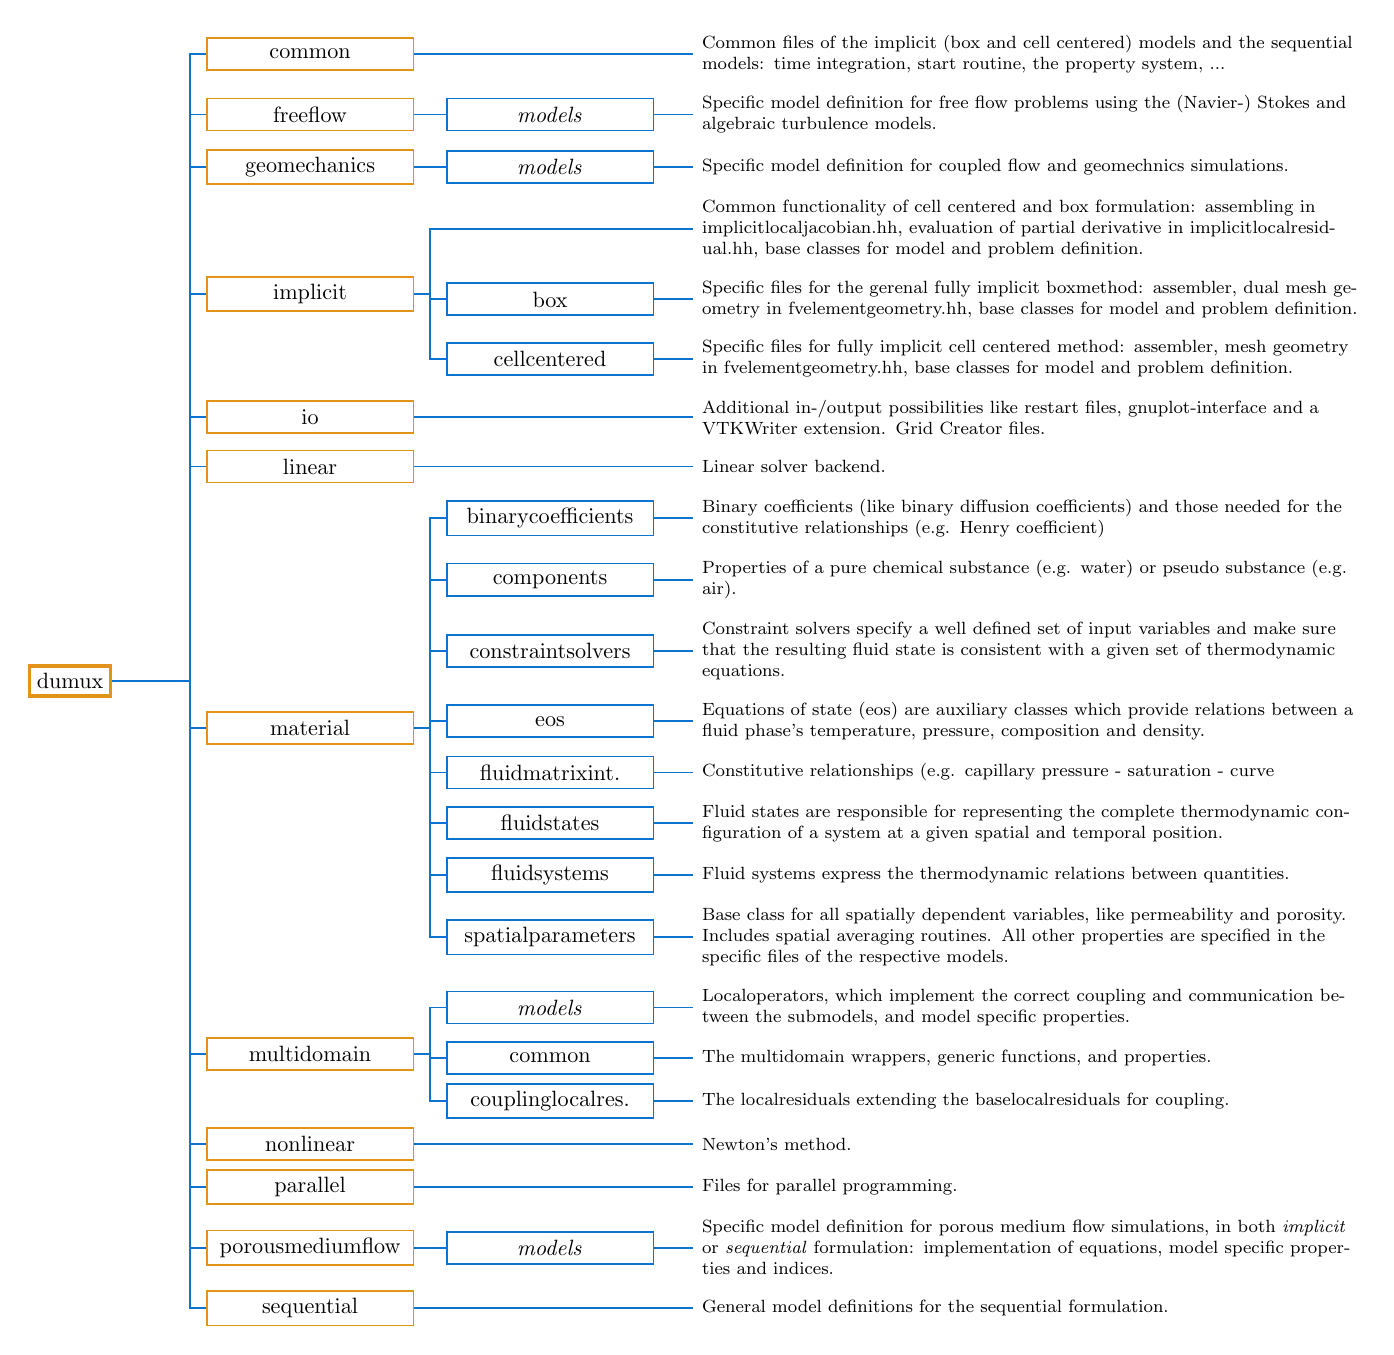
\begin{tikzpicture}[scale=0.8,grow'=right,level distance=1.5in,sibling distance=.05in]
\tikzset{edge from parent/.style={thick, draw=dumuxBlue, edge from parent fork right}}
\tikzset{every tree node/.style={draw, thick, align=center}}
\tikzset{frontier/.style={distance from root=6.0in}}

\tikzset{FirstLevel/.style={
  draw=dumuxYellow,
  rectangle,
  align=center,
  minimum width=1.1in,
  minimum height=0.2in,
  text width=1.2in,
}}
\tikzset{SecondLevel/.style={
  draw=dumuxBlue,
  rectangle,
  align=center,
  minimum width=1.1in,
  minimum height=0.2in,
  text width=1.2in,
}}

\tikzset{ThirdLevel/.style={
  draw=none,
  align=left,
  minimum width=4.2in,
  text width=4.1in,
  font=\footnotesize
}}


\Tree
[.\node[draw=dumuxYellow, ultra thick] {dumux};
  [.\node[FirstLevel] {common};
    \node[ThirdLevel] {
          Common files of the implicit (box and cell centered) models and the
          sequential models: time integration, start routine, the  property
          system, ...};
  ]
  [.\node[FirstLevel] {freeflow};
    [.\node[SecondLevel] {\emph{models}};
      \node[ThirdLevel] {Specific model definition for free flow problems using the (Navier-) Stokes
                         and algebraic turbulence models.};
    ]
  ]
  [.\node[FirstLevel] {geomechanics};
    [.\node[SecondLevel] {\emph{models}};
      \node[ThirdLevel] {Specific model definition for coupled flow and geomechnics simulations.};
    ]
  ]
  [.\node[FirstLevel] {implicit};
%     [.\node[SecondLevel] {\emph{models}};
      \node[ThirdLevel] {Common functionality of cell centered and box formulation:
                         assembling in implicitlocaljacobian.hh, evaluation of partial derivative
                         in implicitlocalresidual.hh, base classes for model and problem definition.};
%     ]
    [.\node[SecondLevel] {box};
      \node[ThirdLevel] {Specific files for the gerenal fully implicit boxmethod:
                         assembler, dual mesh geometry in fvelementgeometry.hh,
                         base classes for model and problem definition.};
    ]
    [.\node[SecondLevel] {cellcentered};
      \node[ThirdLevel] {Specific files for fully implicit cell centered method: assembler,
                         mesh geometry in fvelementgeometry.hh, base classes for model and
                         problem definition.};
    ]
  ]
  [.\node[FirstLevel] {io};
    \node[ThirdLevel] {Additional in-/output possibilities like restart files, gnuplot-interface
                       and a VTKWriter extension. Grid Creator files.};
  ]
  [.\node[FirstLevel] {linear};
    \node[ThirdLevel] {Linear solver backend.};
  ]
  [.\node[FirstLevel] {material};
    [.\node[SecondLevel] {binarycoefficients};
      \node[ThirdLevel] {Binary coefficients (like binary diffusion coefficients) and those
                         needed for the constitutive relationships (e.g. Henry coefficient)};
    ]
    [.\node[SecondLevel] {components};
      \node[ThirdLevel] {Properties of a pure chemical substance (e.g. water)
                         or pseudo substance (e.g. air).};
    ]
    [.\node[SecondLevel] {constraintsolvers};
      \node[ThirdLevel] {Constraint solvers specify a well defined set of input variables
                         and make sure that the resulting fluid state is consistent with a
                         given set of thermodynamic equations.};
    ]
    [.\node[SecondLevel] {eos};
      \node[ThirdLevel] {Equations of state (eos) are auxiliary classes which provide
                         relations between a fluid phase's temperature, pressure, composition
                         and density.};
    ]
    [.\node[SecondLevel] {fluidmatrixint.};
      \node[ThirdLevel] {Constitutive relationships (e.g. capillary pressure - saturation - curve};
    ]
    [.\node[SecondLevel] {fluidstates};
      \node[ThirdLevel] {Fluid states are responsible for representing the complete thermodynamic
                         configuration of a system at a given spatial and temporal position.};
    ]
    [.\node[SecondLevel] {fluidsystems};
      \node[ThirdLevel] {Fluid systems express the thermodynamic relations between quantities.};
    ]
    [.\node[SecondLevel] {spatialparameters};
      \node[ThirdLevel] {Base class for all spatially dependent variables, like permeability and
                         porosity. Includes spatial averaging routines. All other properties are
                         specified in the specific files of the respective models.};
    ]
  ]
  [.\node[FirstLevel] {multidomain};
    [.\node[SecondLevel] {\emph{models}};
      \node[ThirdLevel] {Localoperators, which implement the correct coupling and
                         communication between the submodels, and model specific properties.};
    ]
    [.\node[SecondLevel] {common};
      \node[ThirdLevel] {The multidomain wrappers, generic functions, and properties.};
    ]
    [.\node[SecondLevel] {couplinglocalres.};
      \node[ThirdLevel] {The localresiduals extending the baselocalresiduals for coupling.};
    ]
  ]
  [.\node[FirstLevel] {nonlinear};
    \node[ThirdLevel] {Newton's method.};
  ]
  [.\node[FirstLevel] {parallel};
    \node[ThirdLevel] {Files for parallel programming.};
  ]    
  [.\node[FirstLevel] {porousmediumflow};
    [.\node[SecondLevel] {\emph{models}};
    \node[ThirdLevel] {Specific model definition for porous medium flow simulations, 
                       in both \emph{implicit} or \emph{sequential} formulation: 
                       implementation of equations,
                       model specific properties and indices.};
    ]
  ]
  [.\node[FirstLevel] {sequential};
%     [.\node[SecondLevel] {\emph{models}};
      \node[ThirdLevel] {
           General model definitions for the sequential formulation.};
%     ]
  ]
]
\end{tikzpicture}
\caption{Structure of the directory \texttt{dumux} containing the \Dumux source files.}
\label{fig:dumux-structure}
% \end{sidewaysfigure}
\end{figure}

\section{Setup of new Folders and new Tests}
\label{sc_newfoldersetup}
This section describes how to set up a new folder and how to tell
the build system there is a new one.
\paragraph{Adding new Folders}
\begin{enumerate}[1)]
 \item create new folder with content
 \item adapt the \verb+CMakeList.txt+ in the folder above and add a line with
       \verb+add_subdirectory(NEW_FOLDER)+
 \item create a \verb+CMakeList.txt+ in the newly created folder
 \item go to your \texttt{build}-directory and type \verb+make+ to
       re-configure the system
\end{enumerate}

\paragraph{Adding new Test Programs}
\noindent To add a test use the \texttt{add\_dumux\_test} macro.
The command has four arguments:
\begin{enumerate}[1)]
  \item name of test (has to be unique)
  \item name of executable
  \item source file (*.cc)
  \item command to be executed as test - either the executable or a
        some helper script with arguments
\end{enumerate}

\section{Parameters in \Dumux}
\label{sc_parameterfiles}
Simulation parameters can be parsed to the program via a parameter file or the command line.
A list of all available parameters is provided in the Doxygen documentation
of the file \texttt{parameterfile}, which is accessible via \texttt{Modules -> Parameters}.

After having run the example application from section \ref{quick-start-guide} you will
get the following output at the end of the simulation run
\footnote{If you did not get the output, restart the application the following way:
\texttt{./test{\_}box2p -PrintParameters true},
this will print the parameters once your simulation is finished}:
\begin{lstlisting}[style=Bash]
# Run-time specified parameters:
[ Grid ]
File = "./grids/test_2p.dgf"
[ Implicit ]
EnableJacobianRecycling = "1"
EnablePartialReassemble = "1"
[ Problem ]
Name = "lensbox"
[ SpatialParams ]
LensLowerLeftX = "1.0"
LensLowerLeftY = "2.0"
LensUpperRightX = "4.0"
LensUpperRightY = "3.0"
[ TimeManager ]
DtInitial = "250"
TEnd = "3000"
# DEPRECATED run-time specified parameters:
PrintParameters = "1"
# Replace by:
[ TimeManager ]
PrintParameters = "1"
# Compile-time specified parameters:
[ Implicit ]
EnableHints = "0"
MassUpwindWeight = "1"
MaxTimeStepDivisions = "10"
MobilityUpwindWeight = "1"
NumericDifferenceMethod = "1"
UseTwoPointFlux = "0"
[ LinearSolver ]
MaxIterations = "250"
PreconditionerRelaxation = "1"
ResidualReduction = "1e-06"
Verbosity = "0"
[ Newton ]
WriteConvergence = "0"
[ Problem ]
EnableGravity = "1"
[ TimeManager ]
MaxTimeStepSize = "1.79769e+308"
[ Vtk ]
AddVelocity = "0"
# UNUSED parameters:
ImportantVariable = "1"
\end{lstlisting}

A number of things can be learned:
\begin{itemize}
  \item \emph{run-time} parameters can be changed without re-compiling
  \item \emph{deprecated run-time} parameters will be removed in the next release
  \item \emph{compile-time} parameters cannot be overwritten by the input file
  \item \emph{unused} are not used by the simulation (maybe typo or wrong group)
\end{itemize}

All applications have a help message which you can read by giving
\texttt{--help} as a command line argument to the application.

For further details, please have a look for \texttt{Dune::ParameterTree}
in the \Dune documentation.

\section{Restart \Dumux Simulations}
\label{sec:restartSimulations}

Using the restart capability of \Dumux can be advantageous for computationally
expensive or time consuming simulations, because you can restart the simulation
from a specific point in time and e.g. extend the simulation beyond the originally
end of simulation. What you need is a \texttt{*.drs} file (which contains the
all necessary restart information.
Then you can simply restart a simulation via
\begin{lstlisting}[style=Bash]
./test_program -ParameterFile test_program.input -TimeManager.Restart RESTART_TIME
\end{lstlisting}
To the test restart behavior e.g. use the \texttt{test\_box1p2cni} problem
in the \texttt{test/implicit/1p2c} folder.
You get the \texttt{RESTART\_TIME} from the name of your \texttt{.drs} file.
Please note, that restarting will only work by giving a exact time from
an existing restart file.
Depending on your type of model, you should get a \texttt{.drs} file every
5th or 10th time step. If this not frequently enough, you can change it
by using the following function into your problem header:
\begin{lstlisting}[style=DumuxCode]
/*!
 * \brief Returns true if a restart file should be written to
 *        disk.
 */
bool shouldWriteRestartFile() const
{
  return true;
}
\end{lstlisting}


\input{4_developingdumux}
\section{External Tools}
\label{sc_externaltools}

\subsection{Subversion (svn)}
Subversion is a software versioning and revision control system. We use Subversion to
manage the source code of \Dumux, archive changes and central storage.
Basic svn commands are:
\begin{itemize}
  \item \texttt{svn add} to add files/folder to the repository.
        Use \texttt{svn add --depth=empty FOLDER} to add just the folder
        and \texttt{svn add YOURFILES} to add files. Generally, you should only add
        necessary text-based files. Please do not upload (large) binary files.
  \item \texttt{svn checkout} checkout a repository
  \item \texttt{svn update} updates files/folder
  \item \texttt{svn status} to track changes:
        \textbf{M}odified, \textbf{D}eleted, \textbf{A}dded, \textbf{?} not in repository
  \item \texttt{svn diff} to see the actual changes of files/folder
  \item \texttt{svn commit} upload changes to the repository
\end{itemize}
There are also tools providing a graphical user interface, like \emph{kdesvn} or \emph{eclipse}.

\subsection{Git}
Git is an other version control tool which is currently used to manage the \Dune modules.
The basic Git commands are:
\begin{itemize}
  \item \texttt{git checkout} receive a specified branch from the repository
  \item \texttt{git clone} clone a repository (similar to svn checkout)
  \item \texttt{git diff} to see the actual changes of a file/folder
  \item \texttt{git pull} pull changes from the repository (similar to svn update)
  \item \texttt{git status} to check which files/folders have been changed
\end{itemize}

\subsection{Eclipse}
There is an eclipse style file which can be used for Dumux.
\begin{enumerate}
  \item in eclipse open: \texttt{Window} $\rightarrow$ \texttt{Preferences} $\rightarrow$
        \texttt{C/C++}  $\rightarrow$ \texttt{Code Style} $\rightarrow$ \texttt{Formatter}
  \item press the \texttt{Import} button
  \item choose the file \texttt{eclipse\_profile.xml} from your dumux-devel directory
  \item make sure that that now \Dumux is chosen in \texttt{Select a profile}
\end{enumerate}

\subsection{Kate}
For kate there is syntax highlighting style for \Dumux input files. Simply
copy the file \texttt{dumux-devel/dumuxInputFiles.xml} to the \texttt{syntax} folder in
your kate configuration directory (e.g.
\texttt{HOME/.kde4/share/apps/katepart/syntax/dumuxInputFiles.xml}).

\subsection{ParaView}
\paragraph{Reload Button:}
There are scripts to reload \texttt{*.pvd} or series of {\texttt{*.vtu} files since ParaView 4.2.
The scripts can be found
\href{http://markmail.org/message/exxynsgishbvtngg#query:+page:1+mid:rxlwxs7uqrfgibyv+state:results}{\texttt{under this lin}}.
Just save the specific code portion in a file and load it via \texttt{Macros} $\rightarrow$ \texttt{Add new macro}.

\paragraph{Guide:}
Since ParaView 4.3.1 The ParaView Guide is partly
available for free download, see \url{http://www.paraview.org/documentation/}.
It corresponds to the ParaView book, only without three application chapters.
Attention, its size is 180 MiB.

\input{4_assemblinglinearsystem}

\chapter{Advanced \Dumux\ -- Detailed Instructions}
This chapter contains detailed information for those who are interested
in deeper modifications of underlying \Dumux models, classes, functions, etc.
\section{Models}
Here the basic definitions, the general models concept, and a list of
models available in \Dumux are given.

\subsection{Basic Definitions and Assumptions}
The basic definitions and assumptions are made, using the example
of a three-phase three-component system water-NAPL-gas
\cite{A3:class:2002a}. The modification for other multicomponent
systems is straightforward and can be found, e.\ g., in
\cite{A3:bielinski:2006,A3:acosta:2006}.

\begin{description}
\item[Components:]
The term \emph{component} stands for constituents of the phases which
can be associated with a unique chemical species, or, more generally, with
a group of species exploiting similar physical behavior. In this work, we
assume a water-gas-NAPL system composed of the phases water (subscript
$\text{w}$), gas ($\text{g}$), and NAPL ($\text{n}$). These phases are
composed of the components water (superscript $\text{w}$), the pseudo-component
air ($\text{a}$), and the organic contaminant ($\text{c}$) (see Fig.
\ref{fig:phaseMassEnergyTransfer}).

\item[Phases:]
For compositional multi-phase models, \emph{phases}
are not only matter of a single chemical substance. Instead, their
composition in general includes several species/components. For mass transfer,
the component behavior is quite different from the phase behavior.

\item[Equilibrium:]
For the non-isothermal, multi-phase, multi-component processes in porous media
we state that the assumption of \emph{local thermodynamic equilibrium}.
Chemical equilibrium means that the mass/mole fractions of a component in
different phases are in equilibrium.
Thermal equilibrium assumes the same temperature for all considered phases.
Mechanical equilibrium is not valid in a porous medium, since discontinuities
in pressure can occur across a fluid-fluid interface due to capillary effects.

\item[Notation:]
The subscript index $\alpha \in \{\text{w}, \text{n}, \text{g}\}$ refers
to the phase, while the superscript $\kappa \in \{\text{w}, \text{a}, \text{c}\}$
refers to the component.
\end{description}

\begin{table}
\begin{tabular}{llll}
$p_\alpha$ & phase pressure & $\phi$ & porosity \\
$T$ & temperature & $K$ & absolute permeability tensor \\
$S_\alpha$ & phase saturation & $\tau$ & tortuosity \\
$x_\alpha^\kappa$ & mole fraction of component $\kappa$ in phase $\alpha$ & $\boldsymbol{g}$ & gravitational acceleration \\
$X_\alpha^\kappa$ & mass fraction of component $\kappa$ in phase $\alpha$ & $q^\kappa_\alpha$ & volume source term of $\kappa$ in $\alpha$ \\
$\varrho_{\text{mol},\alpha}$ & molar density of phase $\alpha$ & $u_\alpha$ & specific internal energy \\
$\varrho_{\alpha}$ & mass density of phase $\alpha$ & $h_\alpha$ & specific enthalpy \\
$M$ & molar mass of a phase or component & $c_\text{s}$ & specific heat enthalpy \\
$k_{\text{r}\alpha}$ & relative permeability & $\lambda_\text{pm}$ & heat conductivity \\
$\mu_\alpha$ & phase viscosity & $q^h$ & heat source term \\
$D_\alpha^\kappa$ & diffusivity of component $\kappa$ in phase $\alpha$ & $\boldsymbol{v}_{a,\alpha}$  & advective velocity \\
$\boldsymbol{v}_\alpha$ & velocity (Darcy or free flow)& & \\
\end{tabular}
\caption{Notation list for most of the variables and indices used in \Dumux.}

\end{table}

\begin{figure}
  \centering
  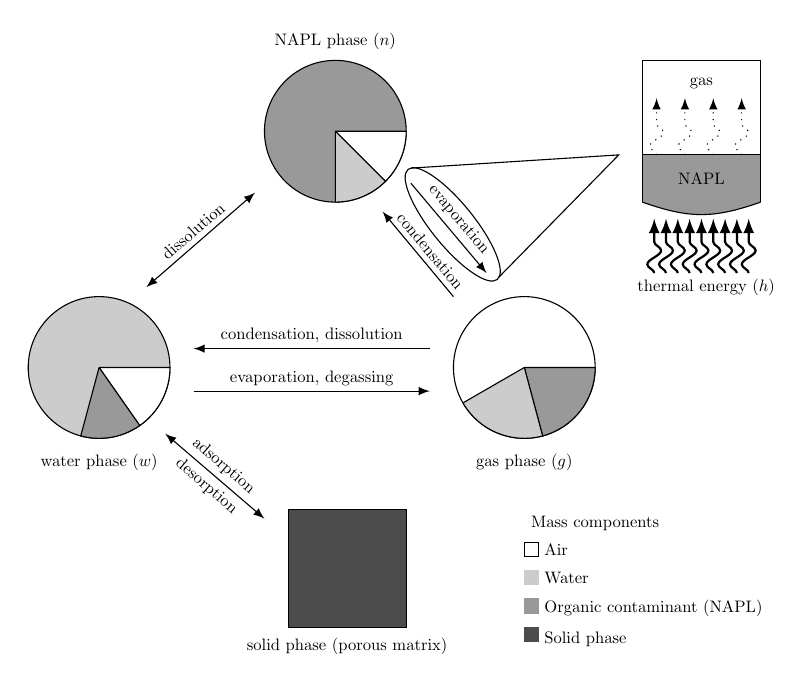
\begin{tikzpicture} [>=latex,scale=0.6, every node/.style={transform shape}]
    % Ellipse 1 solid
    \coordinate (A) at (1,-0.5);
    \draw [fill=black!70](A) rectangle(3.5,2) node at(2.25,-0.9) {solid phase (porous matrix)};
    % Ellipse 2 water
    \coordinate (B) at (-3,5);
    \draw [fill=black!20](B) circle(1.5cm);
    \node [yshift=5mm]at(-3,2.5){water phase $(w)$};
    \draw[fill=white] (B)--+(1.5,0)arc(0:-55:1.5cm)--(B);
    \draw[fill=black!40] (B)--+(-55:1.5cm)arc(-55:-105:1.5cm)--(B);
    % Ellipse 3 gas
    \coordinate (C) at (6,5);
    \draw [](C) circle (1.5cm);
    \node[yshift=5mm]at(6,2.5){gas phase $(g)$};
    \draw [fill=black!40](C)--+(1.5,0)arc(0:-75:1.5cm)--(C);
    \draw [fill=black!20] (C)--+(-75:1.5cm)arc(-75:-150:1.5cm)--(C);
    % Ellipse 4 napl
    \coordinate (D) at (2,10);
    \draw [fill=black!40](D) circle (1.5cm);
    \node[yshift=5mm]at(2,11.4){NAPL phase $(n)$};
    \draw [fill=white](D)--+(1.5,0)arc(0:-45:1.5cm)--(D);
    \draw [fill=black!20] (D)--+(0,-1.5)arc(-90:-45:1.5cm)--(D);
    % arrows
    %A-B
      \draw [<->,white](0.5,1.8)--(-1.6,3.6) node[black,above,sloped,pos=0.5]{adsorption};
      \draw [<->](0.5,1.8)--(-1.6,3.6) node[below,sloped,pos=0.5]{desorption};
    %B-C
      \draw[<-](-1,5.4)--(4,5.4)node[above,sloped,pos=0.5]{condensation, dissolution};
      \draw[->](-1,4.5)--(4,4.5)node[above,sloped,pos=0.5]{evaporation, degassing};
    %B-D
      \draw[<->](-2,6.7)--(0.3,8.7)node[above,sloped,pos=0.5]{dissolution};
    %D-C
      \draw[->](3.6,8.9)--(5.2,7)node[above,sloped,pos=0.5]{evaporation};
      \draw[rotate around={-51:(4,6.8)}](3.35,7.95) ellipse (1.5cm and 0.45cm);  %Ellipse um evaporation
      \draw (3.6,9.22)--(8,9.5)--(5.45,6.9);
      \draw[<-](3,8.3)--(4.5,6.5)node[above,sloped,pos=0.55]{condensation};
    % thermal energy
    \filldraw [black!40](8.5,9.5)rectangle(11,8.5);
    \draw (8.5,9.5)rectangle(11,11.5);
    \draw (8.5,9.5)--(8.5,8.5);
    \draw (11,9.5)--(11,8.5);
    \draw [decorate,decoration={bent,aspect=0.4,amplitude=6},fill=black!40](11,8.5)--(8.5,8.5);
    \foreach \x in {8.75,9,...,10.8}
    \draw [->,decorate,decoration={snake,post length=2mm},thick](\x,7)--(\x,8.15);
    \foreach \x in {8.8,9.4,10,10.6}
    \draw [->,dotted,decorate,decoration={snake,post length=2mm}](\x,9.5)--(\x,10.7);
    \node at(9.75,11){gas};
    \node at(9.75,9){NAPL};
    \node at(9.85,6.7){thermal energy $(h)$};
    % legende
    \node at (7.5,1.7){Mass components};
    \draw[](6,1)rectangle +(0.3,0.3) node at(6.3,1.15) [right]{Air};
    \filldraw[black!20](6,0.4) rectangle +(0.3,0.3) node at (6.3,0.55)[black,right]{Water};
    \filldraw[black!40](6,-0.2) rectangle +(0.3,0.3) node at (6.3,-0.1)[right,black]{Organic contaminant (NAPL)};
    \filldraw[black!70](6,-0.8) rectangle +(0.3,0.3) node at (6.3,-0.75)[right,black]{Solid phase};
  \end{tikzpicture}
  \caption{Mass and energy transfer between the phases}
  \label{fig:phaseMassEnergyTransfer}
\end{figure}



\subsection{Available Models}
We distinguish fully-implicit and sequential models. A list of all available models can be found
in the Doxygen documentation at
\url{http://www.dumux.org/doxygen-stable/html-2.8/modules.php}.
The documentation includes a detailed description for every model.

\subsubsection{Fully-Implicit Models}
The fully-implicit models are using the box or the
cell-centered finite volume method as described in section \ref{box} and \ref{cc}
for spatial and the implicit Euler
method as temporal discretization. The models are located in
subdirectories of \texttt{dumux/implicit}.

\subsubsection{Sequential Models}
The basic idea of the sequential models is to reformulate the
equations of multi-phase flow into one equation for
pressure and equations for phase/component/... transport. The pressure equation
is the sum of the mass balance equations and thus considers the total flow of the
fluid system. The new set of equations is considered as decoupled (or weakly coupled)
and can thus be solved sequentially. The most popular sequential model is the
fractional flow formulation for two-phase flow which is usually implemented applying
an IMplicit Pressure Explicit Saturation algorithm (IMPES).
In comparison to a fully implicit model, the sequential structure allows the use of
different discretization methods for the different equations. The standard method
used in the sequential models is a cell-centered finite volume method. Further schemes,
so far only available for the two-phase pressure equation, are cell-centered finite
volumes with multi-point flux approximation (MPFA O-method) and mimetic finite differences.

An $h$-adaptive implementation of both sequential models is provided for two dimensions.

\section{Spatial Discretization Schemes}
\label{spatialdiscretization}

We discretize space with the cell-centered finite volume method (\ref{cc} ), the box method (\ref{box})
or a staggered grid scheme.
Grid adaption is available for both box and cell-centered finite volume method.
In general, the spatial  parameters, especially the porosity, have to be assigned on
the coarsest level of discretization.

\subsection{Box Method -- A Short Introduction}\label{box}

The so called box method unites the advantages of the finite-volume (FV) and
finite-element (FE) methods.

First, the model domain $\Omega$ is discretized with a FE mesh consisting of nodes
$i$ and corresponding elements $E_k$. Then, a secondary FV mesh is constructed
by connecting the midpoints and barycenters of the elements surrounding node
$i$ creating a box $B_i$ around node $i$ (see Figure \ref{pc:box}a).

\begin{figure} [ht]
\includegraphics[width=0.8\linewidth,keepaspectratio]{png/box_disc.png}
\caption{\label{pc:box} Discretization of the box method}
\end{figure}

The FE mesh divides the box $B_i$ into subcontrolvolumes (scv's) $b^k_i$
(see Figure \ref{pc:box}b). Figure \ref{pc:box}c shows the finite element $E_k$
and the scv's $b^k_i$ inside $E_k$, which belong to four different boxes $B_i$.
Also necessary for the discretization are the faces of the subcontrolvolumes (scvf's)
$e^k_{ij}$ between the scv's $b^k_i$ and $b^k_j$, where $|e^k_{ij}|$ is the length
of the scvf. The integration points $x^k_{ij}$ on $e^k_{ij}$ and the outer normal
vector $\mathbf n^k_{ij}$ are also to be defined (see Figure \ref{pc:box}c).

The advantage of the FE method is that unstructured grids can be used, while the
FV method is mass conservative. The idea is to apply the FV method (balance of
fluxes across the interfaces) to each FV box $B_i$  and to get the fluxes across
the interfaces $e^k_{ij}$ at the integration points $x^k_{ij}$ from the FE approach.
Consequently, at each scvf the following expression results:

\begin{equation}
 	f(\tilde u(x^k_{ij})) \cdot \mathbf n^k_{ij} \: |e^k_{ij}| \qquad \textrm{with}
 	\qquad \tilde u(x^k_{ij}) = \sum_i N_i(x^k_{ij}) \cdot \hat u_i .
\end{equation}

In the following, the discretization of the balance equation is going to be derived.
From the \textsc{Reynolds} transport theorem follows the general balance equation:

\begin{equation}
	\underbrace{\int_\Omega \frac{\partial}{\partial t} \: u \: dx}_{1}
	+ \underbrace{\int_{\partial\Omega} (\mathbf{v} u + \mathbf w) \cdot \textbf n \: d\varGamma}_{2} = \underbrace{\int_\Omega q \: dx}_{3}
\end{equation}

\begin{equation}
	f(u) = \int_\Omega \frac{\partial u}{\partial t} \: dx + \int_{\Omega} \nabla \cdot
	\underbrace{\left[  \mathbf{v} u + \mathbf w(u)\right] }_{F(u)}  \: dx - \int_\Omega q \: dx = 0
\end{equation}
where term 1 describes the changes of entity $u$ within a control volume over
time, term 2 the advective, diffusive and dispersive fluxes over the interfaces
of the control volume and term 3 is the source and sink term. $\Omega$ denotes the
model domain and $F(u) = F(\mathbf v, p) = F(\mathbf v(x,t), p(x,t))$.

Like the FE method, the box method follows the principle of weighted residuals.
In the function $f(u)$ the unknown $u$ is approximated by discrete values at the
nodes of the FE mesh $\hat u_i$ and linear basis functions $N_i$ yielding an
approximate function $f(\tilde u)$. For $u\in \lbrace \mathbf v, p, x^\kappa \rbrace$
this means:

\begin{minipage}[b]{0.47\textwidth}
\begin{equation}
\label{eq:p}
	\tilde p = \sum_i N_i \hat{p}_i
\end{equation}
\begin{equation}
\label{eq:v}
	\tilde{\mathbf v} = \sum_i N_i \hat{\mathbf v}_i
\end{equation}
\begin{equation}
\label{eq:x}
	\tilde x^\kappa  = \sum_i N_i \hat x_i^\kappa
\end{equation}
\end{minipage}
\hfill
\begin{minipage}[b]{0.47\textwidth}
\begin{equation}
\label{eq:dp}
	\nabla \tilde p = \sum_i \nabla N_i \hat{p}_i
\end{equation}
\begin{equation}
\label{eq:dv}
	\nabla \tilde{\mathbf v} = \sum_i \nabla N_i \hat{\mathbf v}_i
\end{equation}
\begin{equation}
\label{eq:dx}
	\nabla \tilde x^\kappa  = \sum_i \nabla N_i \hat x_i^\kappa .
\end{equation}
\end{minipage}

Due to the approximation with node values and basis functions the differential
equations are not exactly fulfilled anymore but a residual $\varepsilon$ is produced.

\begin{equation}
	f(u) = 0  \qquad \Rightarrow \qquad f(\tilde u) = \varepsilon
\end{equation}

Application of the principle of weighted residuals, meaning the multiplication
of the residual $\varepsilon$ with a weighting function $W_j$  and claiming that
this product has to vanish within the whole domain,

\begin{equation}
	\int_\Omega W_j \cdot \varepsilon \: \overset {!}{=} \: 0 \qquad \textrm{with} \qquad \sum_j W_j =1
\end{equation}
yields the following equation:

\begin{equation}
	\int_\Omega W_j \frac{\partial \tilde u}{\partial t} \: dx + \int_\Omega W_j
	\cdot \left[ \nabla \cdot F(\tilde u) \right]  \: dx - \int_\Omega W_j
	\cdot q \: dx = \int_\Omega W_j \cdot \varepsilon \: dx \: \overset {!}{=} \: 0.	
\label{eq:weightedResidual}	
\end{equation}

For standard Galerkin schemes, the weighting functions $W_j$ are chosen the same as the ansatz functions $N_j$. However, this does not yield a locally mass-conservative scheme. 
Therefore, for the Box method, the weighting functions $W_j$ are chosen as 
the piecewise constant functions over a
control volume box $B_j$, i.e.

\begin{equation}
	W_j(x) = \begin{cases}
	          1 &x \in B_j \\
		  0 &x \notin B_j.\\
	         \end{cases}
\label{eq:weightingFunctions}	         
\end{equation}
Thus, the Box method is a Petrov-Galerkin scheme, where the weighting functions do not belong to the same function space than the ansatz functions.

Inserting definition \eqref{eq:weightingFunctions} into equation \eqref{eq:weightedResidual} and using the \textsc{Green-Gaussian} integral theorem results in
\begin{equation}
	\int_{B_j} \frac{\partial \tilde u}{\partial t} \: dx + \int_{\partial B_j}  F(\tilde u) \cdot \mathbf n \: d\varGamma_{B_j} - \int_{B_j} q \: dx  \overset {!}{=} \: 0, 	
\label{eq:BoxMassBlance}	
\end{equation}
which has to hold for every box $B_j$. 

The first term in equation \eqref{eq:BoxMassBlance} can be written as
\begin{equation}
\int_{B_j} \frac{\partial \tilde u}{\partial t} \: dx = \frac{d}{dt} \int_{B_j} \sum_i \hat u_i N_i  \: dx = \sum_i \frac{\partial \hat u_i}{\partial t} \int_{B_j}  N_i  \: dx.
\end{equation} 
Here, a mass lumping technique is applied by assuming that the storage capacity is
reduced to the nodes. This means that the integrals $M_{i,j} = \int_{B_j}  N_i \: dx$
are replaced by some mass lumped terms $M^{lump}_{i,j}$ which are defined as
\begin{equation}
	 M^{lump}_{i,j} =\begin{cases}  V_j &j = i\\
	0 &j \neq i,\\
	         \end{cases}
\end{equation}
where $V_j$ is the volume of the FV box $B_j$ associated with node $j$.
The application of this assumption yields

\begin{equation}
\label{eq:disc1}
	V_j \frac{\partial \hat u_j}{\partial t}
	+  \int_{\partial B_j}  F(\tilde u) \cdot \mathbf n \: d\varGamma_{B_j} - Q_j = 0,
\end{equation}
where $Q_j$ is an approximation (using some quadrature rule) of the integrated source/sink term $\int_{B_j} q \: dx$.

Using an implicit Euler time discretization finally
leads to the discretized form which will be applied to the mathematical
flow and transport equations:

\begin{equation}
\label{eq:discfin}
	V_j \frac{\hat u_j^{n+1} - \hat u_j^{n}}{\Delta t}
	+ \int_{\partial B_j}  F(\tilde u^{n+1}) \cdot \mathbf n
	\;  d{\varGamma}_{B_j} - Q_j^{n+1} \: = 0.
\end{equation}
Equation \eqref{eq:discfin} has to be fulfilled for each box $B_j$.

\subsection{Cell Centered Finite Volume Methods -- A Short Introduction}\label{cc}

\begin{figure} [ht]
\centering
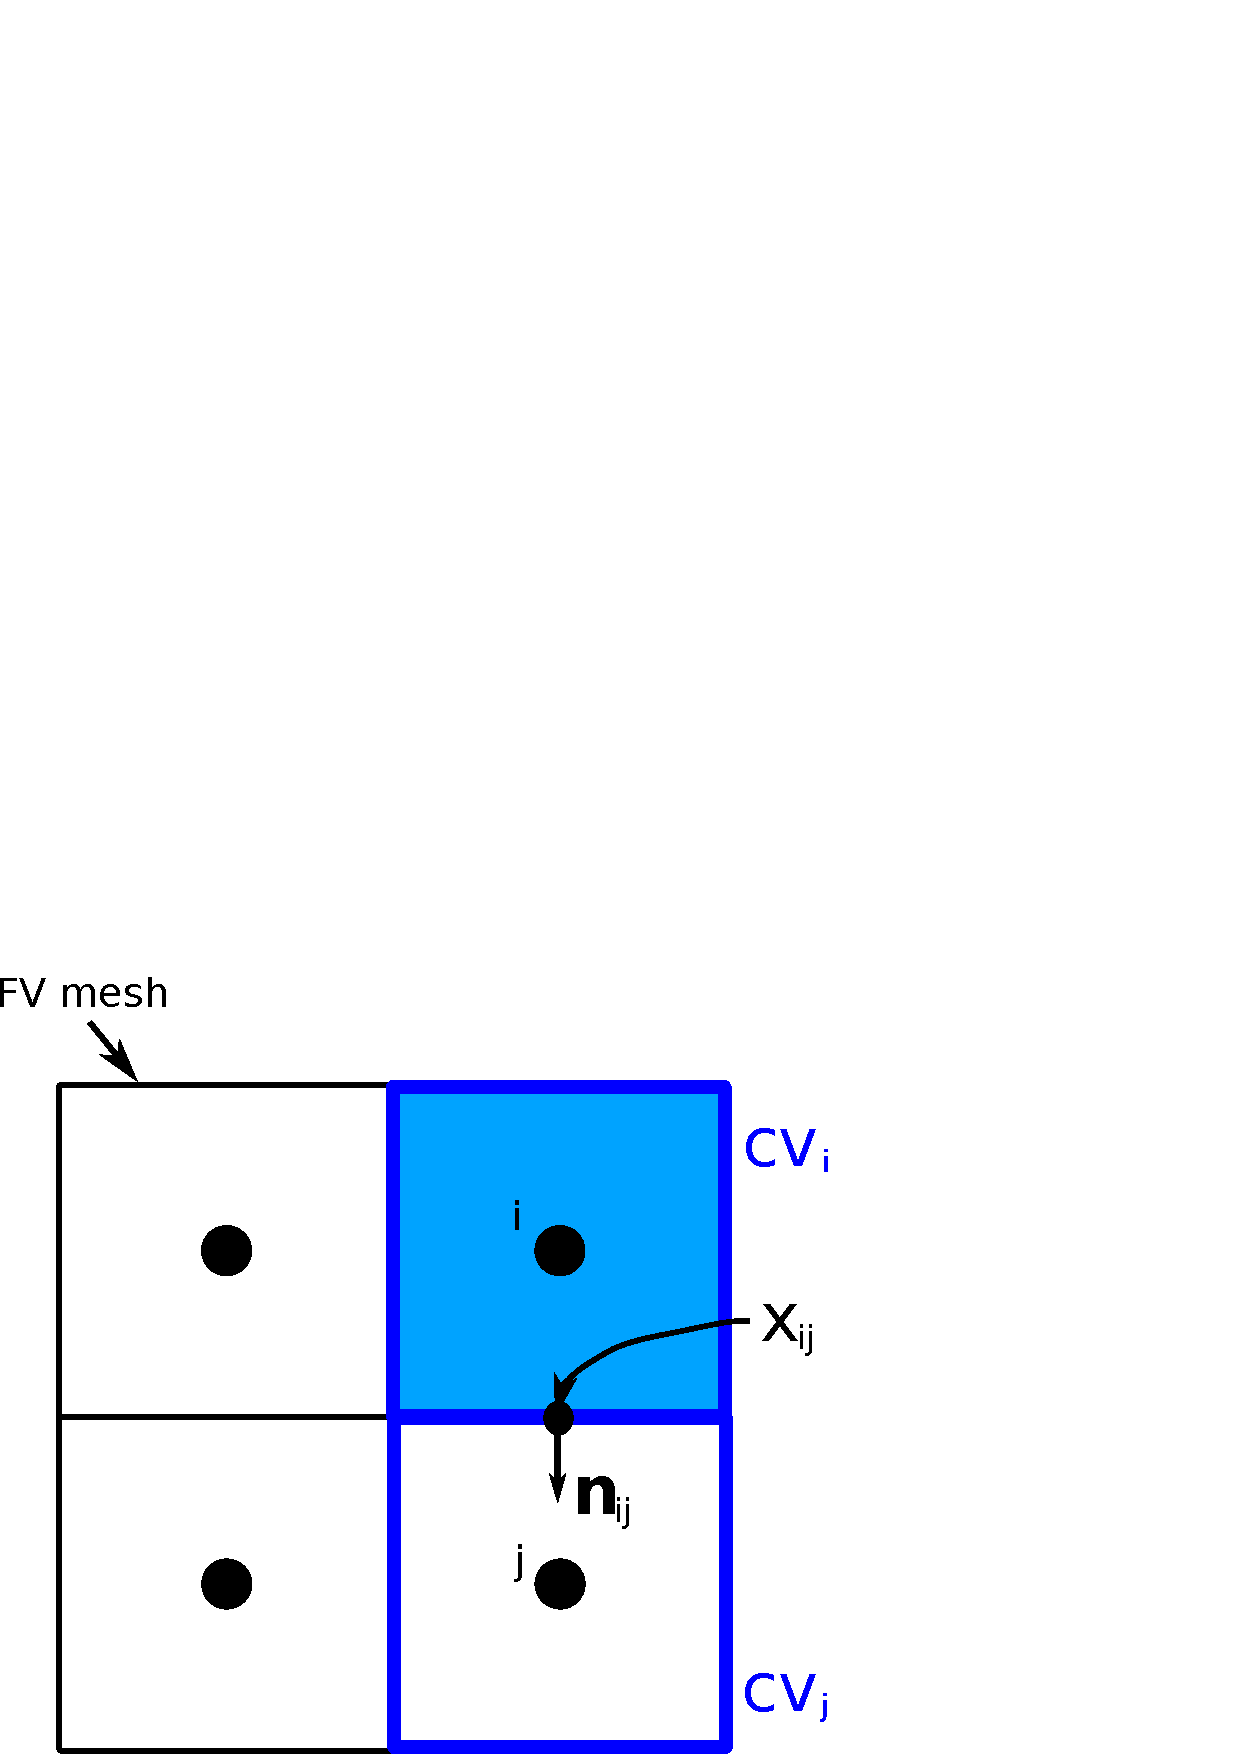
\includegraphics[width=0.4\linewidth,keepaspectratio]{png/cc_disc.png}
\caption{\label{pc:cc} Discretization of the cell centered finite volume method}
\end{figure}

The cell-centered finite volume method uses the elements of the grid as control volumes.
For each control volume all discrete values are determined at the element/control
volume center (see Figure~\ref{pc:cc}).
The mass or energy fluxes are evaluated at the integration points ($x_{ij}$),
which are located at the midpoints of the control
volume faces. This is a two point flux approximation since the flux between
the element/control volume centers $i$ and $j$ is calculated
only with information from these two points. In contrast the box method uses
a multi-point flux approximation where all nodes of the
element influence the flux between two specific nodes. \par
Neumann boundary conditions are applied at the boundary control volume faces
and Dirichlet boundary conditions at the boundary control volumes. \par
The cell centered finite volume method is robust and mass conservative but
should only be applied for structured grids
(the control volume face normal vector ($n_{ij}$) should be parallel to the
direction of the gradient between the two element/control
volume centers).

We consider a domain $\Omega \in \mathbb{R}^d$, $d \in \{ 2, 3 \}$ with boundary $\Gamma = \bar{\Omega} / \Omega$ and the following elliptic model problem:

\begin{equation}
  \begin{aligned}
                   \nabla \cdot \left( - \mathbf{\Lambda} \nabla u \right) &= q   &&\mathrm{in} \, \Omega \\
               \left( - \mathbf{\Lambda} \nabla u \right) \cdot \mathbf{n} &= v_N &&\mathrm{on} \, \Gamma_N \\
                                                                   u &= u_D &&\mathrm{on} \, \Gamma_D.
    \label{eq:elliptic}
  \end{aligned}
\end{equation}

Here, $\mathbf{\Lambda} = \mathbf{\Lambda}(\mathbf{x}, \mathbf{u})$ is a symmetric and positive definite tensor of second rank, $u = u (\mathbf{x})$ is unknown and $q = q(\mathbf{x}, \mathbf{u})$ is a source/sink. For the derivation of the finite-volume formulation we integrate the first equation of \eqref{eq:elliptic} over $\Omega$ and apply the Gauss divergence theorem:

\begin{equation}
    \int_{\Gamma} \left( - \mathbf{\Lambda} \nabla u \right) \cdot \mathbf{n} \mathrm{d} \Gamma = \int_\Omega q \mathrm{d}\Omega.
    \label{eq:ellipticIntegrated}
\end{equation}

We denote by $\mathcal{M}$ the mesh that results from the division of the domain $\Omega$ into $n_e$ control volumes $K_i$. Each $K_i$ is a polygonal open set and $\mathring{K_i} \mathring{\cap K_j} = \emptyset, \forall{i \neq j}$ and $\Omega = \cup_i^{n_e} K_i$. We then enforce equation \eqref{eq:ellipticIntegrated} to be fulfilled in each control volume, which leads to

\begin{equation}
    \sum_{\sigma \in K} F_{K, \sigma} = Q_K, \forall_{K \in \mathcal{M}}
\end{equation}

where $F_{K, \sigma} \approx \int_{\sigma} \left( - \mathbf{\Lambda} \nabla u \right) \cdot \mathbf{n} \mathrm{d} \Gamma$ is the discrete flux through a face $\sigma$ of cell $K$ and $Q_k = \int_K q \mathrm{d}x$ is the integrated source/sink term. 

\subsubsection{TPFA}\label{cc_tpfa}

 

\subsubsection{MPFA}\label{cc_mpfa}
Expressions for the face fluxes $F_{K, \sigma}$ are usually obtained by introducing intermediate face unknowns $\bar{u}_\sigma$ in addition to the cell unknowns $u_K$ and enforcing the physically motivated continuity of fluxes and continuity of the solution across the faces. For a face $\sigma$ between the two polygons $K$ and $L$ these conditions read:

\begin{equation}
    \begin{aligned}
        &F_{K, \sigma} + F_{L, \sigma} = 0 \\
        &\bar{u}_{\sigma, K} = \bar{u}_{\sigma, L} = \bar{u}_{\sigma}.
        \label{eq:sigmaConditions}
    \end{aligned}
\end{equation}

Using these conditions the intermediate face unknowns $\bar{u}_\sigma$ can be eliminated and the fluxes are expressed as a function of the cell unknowns $u_k$ and associated transmissibilities $t_{\sigma, k}$:

\begin{equation}
    F_{\sigma} = \sum_{k \in \mathcal{S}_\sigma} t_{\sigma, k} u_{k}.
    \label{eq:FVFluxExpression}
\end{equation}

%\begin{figure}[t]
%  \hspace{-15mm}
%  \def\svgwidth{500pt}
%  \input{pics/interactionregion.pdf_tex}
%  \caption{Interaction region for the Mpfa-o method. The graphic on the right illustrates %how the sub-control volume $m^v_2$ and face $\sigma^v_2$ are embedded in cell $K_2$. Note %that the face stencils for all sub-control volume faces in the depicted interaction region %are $\mathcal{S}_{\sigma^v_i} = \{ 1, .., 7 \}$.}
%  \label{fig:interactionRegion_mpfa}
%\end{figure}

Here, $\mathcal{S}_\sigma$ is the face stencil. The main difference between the various finite-volume schemes available is the assembly of the face fluxes, i.e.\ the computation of the $t_{\sigma, k}$ and the size of $\mathcal{S}_\sigma$. The standard scheme used in industrial codes is the two-point flux approximation (tpfa), which is computationally very efficient, but leads to inconsistent fluxes on general meshes. We cannot assure certain mesh properties as we want to consider meshes being constrained to arbitrary lower-dimensional fracture entities. Therefore, the method presented in this work is based on a multi-point flux approximation method (Mpfa-o method), which was first introduced in \citet{Aavatsmark2002}. In this scheme, a dual grid is created by connecting the barycenters of the cells with the barycenters of the faces ($d=2$) or the barycenters of the faces and edges ($d=3$). This divides each cell into sub-control volumes $m^v_K$ and each face into sub-control volume faces $\sigma^v$. The continuity conditions \eqref{eq:sigmaConditions} are now imposed on the $\sigma^v$ locally within an interaction region, which consists of sub-cells and sub-control volume faces sharing a common vertex (see fig. \ref{fig:interactionRegion_mpfa}). We allow for piecewise constant $\mathbf{\Lambda}$ (per cell) and construct discrete gradients $\nabla_K^v u$ (per sub-control volume), which enables us to write the discrete flux across $\sigma^v_1$ from cell $1$ as follows:

\begin{equation}
    F_{1, \sigma^v_1} = - |\sigma^v_1| \mathbf{n}_{\sigma^v_1}^T \mathbf{\Lambda}_1 \nabla_1^v u.
    \label{eq:discreteFlux}
\end{equation}

We use the definition for the sub-control volume gradient given in \citet{Aavatsmark2002}:

\begin{equation}
    \nabla_1^v u = \frac{1}{T_1} \boldsymbol{\nu}_{11} (\bar{u}_{\sigma^v_1} - u_1) +
                   \frac{1}{T_1} \boldsymbol{\nu}_{12} (\bar{u}_{\sigma^v_7} - u_1),
\end{equation}

which uses the relations

\begin{equation}
    \begin{aligned}
        &\boldsymbol{\nu}_{11} = \mathbf{R} \mathbf{x}_{12}, \\
        &\boldsymbol{\nu}_{12} = - \mathbf{R} \mathbf{x}_{11}, \\
        &T_1 = \| \mathbf{x}_{12} \mathbf{R} \mathbf{x}_{11} \|,
    \end{aligned}
\end{equation}

where $\mathbf{R} = \left( {\begin{array}{cc}
                                     0 & 1 \\
                                     -1 & 0
                                     \end{array} } \right)$. Inserting this into equation \eqref{eq:discreteFlux} gives

\begin{equation}
    F_{1, \sigma^v_1} = - \frac{|\sigma^v_1| \mathbf{n}_{\sigma^v_1}^T \mathbf{\Lambda}_1 \boldsymbol{\nu}_{11}}{T_1} (\bar{u}_{\sigma^v_1} - u_1) -
                         \frac{|\sigma^v_1| \mathbf{n}_{\sigma^v_1}^T \mathbf{\Lambda}_1 \boldsymbol{\nu}_{12}}{T_1} (\bar{u}_{\sigma^v_7} - u_1).
\end{equation}

We now introduce the coefficients $\omega^k_{j, \sigma_i^v} = - \frac{|\sigma^v_i| \mathbf{n}_{\sigma^v_i}^T \mathbf{\Lambda}_j \boldsymbol{\nu}_{jk}}{T_j}$, where $j$ and $i$ are the local indices of a sub-control volume and sub-control volume face within the interaction region and $k$ ($1 \leq k \leq d$) is the local coordinate direction in the sub-control volume. This leads to the following general expression for a sub-control volume face flux (here shown for $d = 2$)

\begin{equation}
    F_{j, \sigma^v_i} = \left( \omega^1_{j, \sigma^v_i} \hspace{2mm} \omega^2_{j, \sigma^v_i} \right)^T \left( {\begin{array}{c}
                                                                                                                \bar{u}_{\sigma^v_{\varphi(j, 1)}} - u_j \\
                                                                                                                \bar{u}_{\sigma^v_{\varphi(j, 2)}} - u_j
                                                                                                                \end{array} } \right),
\end{equation}

where we introduced the surjective function $\varphi: (j, k) \rightarrow i$, which maps to each pair of local sub-control volume index and coordinate direction the local index of the corresponding sub-control volume face. The fluxes for all sub-control volume faces within an interaction region can be written in matrix form as a function of the $u_j$ and $\bar{u}^v_{\sigma^v_i}$:

\begin{equation}
    \mathbf{f} = \mathbf{C}^{7 \times 7} \mathbf{\bar{u}} + \mathbf{D}^{7 \times 7} \mathbf{u}.
    \label{eq:fluxesInInteractionVolume}
\end{equation}

The continuity conditions \eqref{eq:sigmaConditions} are enforced on one point per sub-control volume face, which can be defined anywhere between the center of the face of the primal grid and the vertex position, parameterized by $q$ ($0 \leq q < 1$, see fig. \ref{fig:interactionRegion_mpfa}). This gives rise to one equation per face, which in matrix form reads

\begin{equation}
    \mathbf{A}^{7 \times 7} \mathbf{\bar{u}} = \mathbf{B}^{7 \times 7} \mathbf{u}
    \label{eq:localSystem}
\end{equation}

and leads to the following expression for the sub-control volume face fluxes as a function of only the cell unknowns $\mathbf{u}$:

\begin{equation}
    \mathbf{f} = \mathbf{C}^{7 \times 7} \mathbf{\bar{u}} + \mathbf{D}^{7 \times 7} \mathbf{u} \
               = \left[ \mathbf{C}^{7 \times 7} \left( \mathbf{A}^{7 \times 7} \right)^{-1} \mathbf{B}^{7 \times 7} + \mathbf{D}^{7 \times 7} \right] \mathbf{u} = \mathbf{T}^{7 \times 7} \mathbf{u}.
    \label{eq:fluxExpression}
\end{equation}

In the above equation \eqref{eq:fluxExpression} the rows of the system are the resulting flux expressions $F_{\sigma^v_i} = \sum_{k = 1}^7 t_{\sigma^v_i, k} u_{k}$ for the sub-control volume faces within the interaction region, where the matrix $\mathbf{T}$ contains the corresponding transmissibilities. The overall flux across a face $\sigma$ of the primal grid is the sum over all its embedded sub-control volume faces:

\begin{equation}
    F_{\sigma} = \sum_{\sigma^v \in \sigma} F_{\sigma^v}.
\end{equation}
% \subsubsection{NLTPFA}\label{cc_nltpfa}
% TODO

\subsection{Staggered Grid -- A Short Introduction}\label{staggered}

\begin{figure}[ht]
\centering
\includegraphics[width=.8\linewidth]{./pdf/staggered_grid.pdf}
\caption{\label{pc:staggered} Discretization of the staggered-grid method. The figure shows the different control volume arrangements, which are staggered with respect to each other. There are the control volumes centered around the scalar primary variables in black, the control volumes located around the $x$-component of the velocity in blue and the control volumes located around the $y$-components of the velocity in red. The control volume boundaries are given by lines. Additionally, there is one shaded example control volume each.\\
In the two-dimensional free-flow models, the continuity equation is discretized using the black control volumes, the $x$-component of the momentum equation is discretized using the blue control volumes and the $y$-component is discretized using the red control volumes. In three dimensions this works analogously.}
\end{figure}

The staggered-grid or marker-and-cell method uses a finite volume method with different control volumes for different equations. There are control volumes centered around the scalar primary variables. They correspond to the finite volume mesh. Additionally, there are control volumes located around the $x,y$ and (in 3D) $z$ velocity components which are shifted in the $x,y$ and $z$ direction, such that the velocity components are located on the edges of the cell-centered finite volume mesh (see Figure~\ref{pc:staggered}). As for the cell-centered method, the fluxes are evaluated at the edges of each control volume with a two-point flux approximation, cf. \ref{cc}.\par
The staggered-grid method is robust, mass conservative, and free of pressure oscillations
but should, as the cell-centered TPFA method, only be applied for structured grids.
Currently, all free-flow models in \Dumux use the staggered-grid discretization.

\section{Steps of a \Dumux Simulation}
\label{flow}


This chapter is supposed to show how things are ``handed around'' in \Dumux. It
is not a comprehenisve guide through the modeling framework of \Dumux, but
hopefully it will help getting to grips with it.

In Section \ref{content} the structure of \Dumux is shown from a \emph{content}
point of view.
Section \ref{implementation} however is written from the point of view of the \emph{implementation}.
The same coloration in the flowcharts of both sections refers to the same level of calculation. For keeping things 
simple, the program flow of a \verb+2p+ model is shown in section \ref{implementation}. There are extensive comments 
regarding the formating in the tex file: so feel free, to enhance this description.

\subsection{Structure -- by Content}

\label{content}
% by means of this enumerated list, the connection between algorithm and content
% can be achieved by references to the labels of this list.
This list shows the algorithmic outline of a typical \Dumux run. Each item stands
for a characteristic step within the modeling framework.

%\clearpage
In Figure \ref{fig:algorithm}, the algorithmic representations of both approaches, the coupled fully 
implicit and the decoupled semi-implicit one are illustrated down to the element level.

\begin{figure}[hbt]
\begin{tabular}{ l | l }

\begin{minipage}[t]{0.48\textwidth}
\setcounter{thingCounter}{0}

\scriptsize
\sffamily
\begin{tabbing}
\textbf{{\begin{turn}{45}\color{black}\numberThis{main}{init}\end{turn}}}             \=
\textbf{{\begin{turn}{45}\color{dumuxBlue}\numberThis{time step}{prep}\end{turn}}}            \=
\textbf{{\begin{turn}{45}\color{Mulberry}\numberThis{\textsc{Newton}}{elem}\end{turn}}}         \=
\textbf{{\begin{turn}{45}\color{dumuxYellow}\numberThis{element}{calc}\end{turn}}}             \=  \\
\\
\color{black}initialize \\
\color{black}\textbf{foreach} time step\\

  \> \color{dumuxBlue}prepare update\\
  \> \color{dumuxBlue}\textbf{foreach} \textsc{Newton} iteration \\

    \> \> \color{Mulberry}\textbf{foreach} element \\

      \> \> \> \color{dumuxYellow}- calculate element \\
      \> \> \> \color{dumuxYellow}\; residual vector and \\
      \> \> \> \color{dumuxYellow}\; Jacobian matrix\\
      \> \> \> \color{dumuxYellow}- assemble into global\\
      \> \> \> \color{dumuxYellow}\; residual vector and \\
      \> \> \> \color{dumuxYellow}\;{Jacobian} matrix \\

    \> \> \color{Mulberry}\textbf{endfor} \\

    \> \> \color{Mulberry}solve linear system\\
    \> \> \color{Mulberry}update solution\\
    \> \> \color{Mulberry}check for \textsc{Newton} convergence\\
  \> \color{dumuxBlue}\textbf{endfor}\\
  \> \color{dumuxBlue}- adapt time step size, \\
  \> \color{dumuxBlue}\; possibly redo with smaller step size\\
  \> \color{dumuxBlue}- write result\\
\color{black}\textbf{endfor}\\
\color{black}finalize
\end{tabbing}

\end{minipage}

&

\begin{minipage}[t]{0.48\textwidth}
\setcounter{thingCounter}{0}

\scriptsize
\sffamily
\begin{tabbing}
\textbf{{\begin{turn}{45}\color{black}1. main\end{turn}}}             \=
\textbf{{\begin{turn}{45}\color{dumuxBlue}2. time step\end{turn}}}            \=
\textbf{{\begin{turn}{45}\color{Mulberry}3. \textsc{IMPES/C}\end{turn}}}        \=
\textbf{{\begin{turn}{45}\color{dumuxYellow}4. element\end{turn}}}             \=  \\
\\
\color{black}initialize \\
\color{black}\textbf{foreach} time step\\

  \> \color{dumuxBlue}prepare update\\
  \> \color{dumuxBlue}\textbf{foreach} \textsc{IMPES/C} step \\
    \> \> \color{Mulberry}\textbf{if} grid is adaptive\\
      \> \> \> \color{dumuxYellow}- calculate refinement indicator\\
      \> \> \> \color{dumuxYellow}- mark elements, adapt the grid\\
      \> \> \> \color{dumuxYellow}- map old solution to new grid\\
    \> \> \color{Mulberry}- calculate {flow field}\\
    \> \> \color{Mulberry}\textbf{foreach} element \\

      \> \> \> \color{dumuxYellow}- calculate element stiffness matrix \\
      \> \> \> \color{dumuxYellow}- assemble into global matrix \\

    \> \> \color{Mulberry} \textbf{endfor} \\
    \> \> \color{Mulberry} solve linear system\\

    \> \> \color{Mulberry}- calculate {transport} \\
    \> \> \color{Mulberry}\; (saturations, concentrations,...) \\
    \> \> \color{Mulberry}\textbf{foreach} element  \\
      \> \> \> \color{dumuxYellow}-calculate update (explicitly) \\
      \> \> \> \color{dumuxYellow}- adapt time step ({CFL}-like criterion) \\
    \> \> \color{Mulberry}\textbf{endfor} \\
    \> \> \color{Mulberry}- update old solution \\
    \> \> \color{Mulberry}- postprocess (flash calculation, etc.)\\
  \> \color{dumuxBlue}\textbf{endfor}\\
  \> \color{dumuxBlue}- write result\\
\color{black}\textbf{endfor}\\
finalize
\end{tabbing}

\end{minipage}
\end{tabular}

\caption{Structure of a coupled fully-implicit (\textbf{left}) and a decoupled
semi-implicit (\textbf{right}) scheme in \Dumux.}
\label{fig:algorithm}
\end{figure}

\subsection{Structure --  by Implementation}
 \label{implementation}
This section is supposed to help you in getting an idea how things are handled in
\Dumux and in which files things are written down.
This is not intuitivly clear, therefore it is mentioned for each \fbox{step-stone}.
\textbf{called by} tells you from which file a function is
accessed. \textbf{implemented in} tells you in which file the function is written
down. The name of the function is set in \verb+typewriter+.
Being a function is indicated by round brackets \verb+()+ but only the function
name is given and not the full signature (arguments...) .
Comments regarding the events within one step-stone are set \scriptsize{smaller}.

\begin{landscape}
\pagestyle{empty} % switch off headings and footer in order to get more space for the flowchart
\setlength{\voffset}{4.2cm}

% command for blocks
\newcommand{\step}[6]{
\begin{minipage}{7.5cm}
{\tiny \color{#1}\texttt{#2} $\Rightarrow$ \texttt{#3}}\\
\fcolorbox{#1}{white}{
    \begin{minipage}{7.0cm}
    \begin{scriptsize}
    \texttt{#4} \hfill \color{gray}in: #5\color{black}\\
    \hphantom{m}\begin{minipage}[t]{6.8cm}#6\end{minipage}
    \end{scriptsize}
    \end{minipage}}
\end{minipage}
}

% command for the arrow with text
\newcommand{\longArrow}[1]{
\begin{minipage}[b]{7.5cm}
\fcolorbox{white}{white}{
\begin{minipage}[b]{7.0cm}
    \begin{center}
    \begin{scriptsize}
    $\overrightarrow{ %an arrow under which things may be written
      \begin{array}{c} % in order to be able to write multiple lines under the arrow
      #1\\
      \hphantom{\hspace{6.5cm}}
      \end{array}
    }$
    \end{scriptsize}
    \end{center}
\end{minipage}%
}
\end{minipage}%
\hphantom{ $\overrightarrow{}$}%
}

% command for the arrow between steps
\newcommand{\shortArrow}{$\overrightarrow{}$}

% command for marking things as model specific
\newcommand{\modelSpecific}{\emph{model specific}\xspace}

% the distance between two lines
\newcommand{\dummyDistance}{\\[4\baselineskip]}

% THE FLOW CHART STARTS HERE
\noindent
\step{black}{main()}{Dumux::start<ProblemTypeTag>() $\Rightarrow$ start\_()}{start\_()}{start.hh}%
     {start the simulation}
\shortArrow
\step{black}{start\_()}{timeManager.init()}{init()}{timemanager.hh}%
     {initialization}
\shortArrow
\step{black}{start\_()}{timeManager.run()}{run()}{timemanager.hh}%
     {time step management}
\dummyDistance
%
\longArrow{
    \textnormal{\texttt{while(!finished)}}\\
    \textnormal{\color{black}main}
    \rightarrow \textnormal{\color{dumuxBlue}time step}
    }
\step{dumuxBlue}{run()}{problem->timeIntegration()}{timeIntegration()}{implicitproblem.hh}%
     {execute time integration scheme}%
\longArrow{
    \textnormal{define number of allowed \textsc{Newton} fails}\\
    \textnormal{(each halving dt)}
    }
\dummyDistance
%
\step{dumuxBlue}{timeIntegration()}{model->update()}{update()}{implicitmodel.hh}%
     {sth like numerical model}
\shortArrow
\step{dumuxBlue}{update()}{solver.execute()}{execute()}{newtonmethod.hh}%
     {applying \textsc{Newton} method\\
      keeps track of things, catching errors}
\longArrow{
    \textnormal{\color{dumuxBlue}time step}
    \rightarrow \textnormal{\color{Mulberry}Newton step}\\
    \texttt{while(ctl.newtonProceed()}\\
    \textnormal{uLastIter = uCurrentIter(model.uCur())}
    }
\dummyDistance
%
\noindent
\step{Mulberry}{execute() $\Rightarrow$ execute\_()}{jacobianAsm.assemble()}{assemble()}{implicitassembler.hh}%
     {linearize the problem:\\
      add all element contributions to global \textsc{Jacobian}
      and global residual}%
\shortArrow
\step{Mulberry}{assemble() $\Rightarrow$ asImp\_().assemble\_()}{resetSystem\_()}{resetSystem\_()}{implicitassembler.hh}%
     {set r.h.s. (i.e. residual)\\
      set \textsc{Jacobian}  to zero }
\longArrow{
    \textnormal{\color{Mulberry}Newton step}
    \rightarrow \textnormal{\color{dumuxYellow}element}\\
    \texttt{loop all elements}\\
    }
\dummyDistance
%
\noindent
\step{dumuxYellow}{assemble() $\Rightarrow$ asImp\_().assemble\_()}{asImp\_().assembleElement\_()}{assembleElement\_()}{e.g. boxassembler.hh}%
     {call local \textsc{Jacobian} and residual assembly}%
\shortArrow
\step{dumuxYellow}{assembleElement\_()}{model\_().localJacobian().assemble()}{assemble()}{implicitlocaljacobian.hh}%
     {set curr. element, update element's fin.vol.geom.\\
      reset local \textsc{Jacobian} to 0\\
      update types of boundaries on this element}%
\shortArrow
\step{dumuxYellow}{assemble()}{prevVolVars\_.update(),curVolVars\_.update()}{update()}{e.g. 2pvolumevariables.hh}%
     {call model (e.g. \texttt{2p})specific update of quantities defined for the volume:\\
      variables for the \emph{current} and \emph{previous} timestep}%
\dummyDistance
%
\noindent
\step{dumuxYellow}{update()}{completeFluidState()}{completeFluidState()}{e.g. 2pvolumevariables.hh}%
     {calculate all required fluid properties from the primary variables,
      here the fluid system does the real work:\\
      calculates, saves, and provides: densities, etc.}
\shortArrow
\step{dumuxYellow}{assemble()}{localResidual().eval()$\Rightarrow$asImp\_().eval()}{eval()}{e.g. implicitlocalresidual.hh}%
     {the element's local residual is calculated:\\
      see the next two stepstones}%
\shortArrow
\step{dumuxYellow}{eval()}{asImp\_().evalFluxes\_()}{evalFluxes\_()}{e.g. boxlocalresidual.hh}%
     {evaluate the fluxes going into each finite volume,
      this is \modelSpecific}
\dummyDistance
%
\step{dumuxYellow}{evalFluxes\_()}{this$\rightarrow$asImp\_().computeFlux()}{computeFlux()}{e.g. 2plocalresidual.hh}%
     {this calculate the \modelSpecific fluxes (e.g. advective and diffusive)
      using the \texttt{FluxVariables}}
\shortArrow
\step{dumuxYellow}{eval()}{asImp\_().evalVolumeTerms\_()}{evalVolumeTerms\_()}{implicitlocalresidual.hh}%
     {evaluate the \modelSpecific storage and source terms for each finite volume}%
\shortArrow
\step{dumuxYellow}{eval()}{asImp\_().evalBoundary\_()}{evalBoundary\_()}{implicitlocalresidual.hh}%
     {evaluate the \modelSpecific boundary conditions}%
\dummyDistance
%
\step{dumuxYellow}{assemble()}{asImp\_().evalPartialDerivative\_()}{evalPartialDerivative\_()}{e.g. implicitlocaljacobian.hh}%
     {actually calculate the element's (local) \textsc{Jacobian}\\
      matrix a property chooses backward/central/foward\\
      differences. here: central differences}
\shortArrow
\begin{minipage}{0.50\textwidth}
  \begin{scriptsize}\textnormal{approximation of partial derivatives: numerical differentiation}\end{scriptsize}\\
  \begin{scriptsize}\textnormal{add $\pm \epsilon$ solution, divide difference of residual by $2\epsilon$}\end{scriptsize}\\
  \begin{scriptsize}\textnormal{all partial derivatives for the element from the local \textsc{Jacobian} matrix}\end{scriptsize}\\
  $\left \lbrace
      \begin{tabular}{l}%these question marks are for the \verb, not meant as ``unclear''
          \verb?priVars[pvIdx]+=eps?\\
          \begin{scriptsize}\textnormal{this is adding eps to the current solution}\end{scriptsize}\\
      \verb?curVolVars_[scvIdx].update(+eps)?\\
          \begin{scriptsize}\textnormal{recalculate volume variables, having $\epsilon$ added}\end{scriptsize}\\
          \verb?localResidual().eval(+eps)?\\
          \begin{scriptsize}\textnormal{calculate local residual for modified solution as before: involves}\end{scriptsize}\\
      {\scriptsize $\begin{array}{l}
          \textnormal{- \textbf{computeFlux}}\\
          \textnormal{- \textbf{computeStorage}}\\
          \textnormal{- \textbf{computeSource}} \\
      \end{array}$} \\
      \verb?store the residual()?\\
      \verb?repeat for priVars[pvIdx]-=eps?\\
      \verb?derivative is (residual(+eps) - residual(-eps))/2eps?\\
    \end{tabular}
    \right .
  $
\end{minipage}
\dummyDistance
%
\step{dumuxYellow}{assemble\_()}{asImp\_().assembleElement\_()}{assembleElement\_()}{implicitassembler.hh}%
     {Residual of the current solution is now\\
      ``numerically differentiated'', for the element i.e.\\
      the local \textsc{Jacobian} matrix is calculated. }%
\longArrow{
    \textnormal{The contribution of a single element is done.}\\
    \textnormal{Now, it needs to be added to the global quantities:}\\
    \textnormal{Add to global residual and global \textsc{Jacobian}}.}
\step{dumuxYellow}{assemble\_()}{asImp\_().assembleElement\_()}{assembleElement\_()}{e.g. boxassembler.hh}
     {Add to global residual.:\\
      \texttt{resdidual\_[globI+=\\model\_().globalJacobian().resdidual(i)]}}
\dummyDistance
%
\longArrow{
    \textnormal{loop vertices}\\
    \textnormal{of an element}
    }
\step{dumuxYellow}{assemble\_()}{asImp\_().assembleElement\_()}{assembleElement\_()}{e.g. boxassembler.hh}
     {Add to global residual:\\
      \texttt{(*matrix\_)[globI][globJ] +=\\model\_().localJacobian().mat(i,j)}}
\longArrow{
    \textbf{\textbf{\color{dumuxYellow}element}}
    \rightarrow \textbf{\color{Mulberry}Newton step}\\
    \textnormal{Assembling of elements to global quantities is done.}
    }
\dummyDistance
%
\step{Mulberry}{execute\_()}{while(ctl.newtonProceed())}{newtonProceed()}{newtoncontroller.hh}%
     {Print information.\\
      Start/ stop timer.}%

\longArrow{
    \textnormal{set delta Vector to zero} \\
    \textnormal{(this is what is}\\
    \textnormal{solved for later)}\\
    }
\step{Mulberry}{execute\_()}{ctl.newtonSolveLinear()}{newtonSolveLinear()}{newtoncontroller.hh}%
     {Catching errors.\\
      Ask the linear solver to solve the system.\\
      i.e.: give \textsc{Jacobian}(matrix), delta(x), r.h.s.(residual) to linear solver\\
      $\nabla r(x^k) \cdot \Delta x^k = r(x^k)$\\
      tricky: each \textsc{Newton} step solves a linear system of equations.}%
\shortArrow
\step{Mulberry}{newtonSolveLinear()}{int converged = linearSolver\_.solve()}{solve()}{boxlinearsolver.hh}%
     {Solve the linear system with the chosen backend.}%
\dummyDistance
%
\step{Mulberry}{execute\_()}{ctl.newtonUpdate()}{newtonUpdate()}{newtoncontroller.hh}%
     {We solved for the change in solution, but need the solution:\\
      Calculate current (this iteration) solution\\
      \quad from last (iteration) solution and current (iteration) change in  solution:\\
      $x^{k+1} = x^k - \Delta x^k$ where $\Delta x^k = (\nabla r(x^k))^{-1} \cdot r(x^k)$}
\shortArrow
\step{Mulberry}{execute\_()}{ctl.newtonEndStep()}{newtonEndStep()}{newtoncontroller.hh}%
     {Increase counter for number of \textsc{Newton} steps.\\
      Print info.}%
\longArrow{
    \textnormal{check whether to do another \textsc{Newton} iteration:} \\
    \textnormal{that is: check if the error is below tolerance or}\\
    \textnormal{maximum number of iterations was reached.}
    }
\dummyDistance
%
\longArrow{
    \textbf{\textbf{\color{Mulberry}Newton step}}
    \rightarrow \textbf{\color{dumuxBlue}Time step}\\
    \textnormal{\textsc{Newton} done}\\
    \textnormal{if failed $\rightsquigarrow$ halve timestep size, restart loop}\\
    }
\step{dumuxBlue}{execute\_()}{ctl.newtonEnd()}{newtonEnd()}{newtoncontroller.hh}%
     {Tell the controller we are done}%
\shortArrow
\step{dumuxBlue}{update()}{asImp\_().updateSuccessful()}{updateSuccessful()}{e.g. implicitmodel.hh}%
     {can be filled \modelSpecific}%
\dummyDistance
%
\longArrow{
    \textnormal{in while(!finished)}
    }
\step{dumuxBlue}{run()}{problem\_->postTimeStep()}{postTimeStep(),writeOutput()}{implicitproblem.hh}%
     {Give the problem the chance to post-process the solution.}%
\longArrow{
    \textnormal{write output}\\
    \textnormal{uPrev $\leftarrow$ uCur}\\
    \textnormal{time += dt, timestepIdx++}\\
    \textnormal{deal with restart and episodes }
    }
\dummyDistance
%
\step{dumuxBlue}{run()$\Rightarrow$setTimeStepSize(problem\_->nextTimeStepSize(dt))\\
                 $\Rightarrow$nextTimeStepSize()}
     {newtonCtl\_.suggestTimestepSize()}{suggestTimestepSize()}{newtoncontroller.hh}%
     {Determine new time step size from number of \textsc{Newton} steps.}%
\longArrow{
  \textbf{\color{dumuxBlue}Time step}
  \rightarrow \textbf{\color{black}main}\\
  \textnormal{loop until simulation is finished}
}

\end{landscape}

\newpage
% Original pagestyle (headings and footer) were switched off,
% in order to get more space for the flowchart.
\pagestyle{scrheadings}
\normalsize

\section{Property System}
\label{sec:propertysystem}
A high level overview over the property system's design and principle ideas
are given, then follows a reference and a self-contained example.

\subsection{Motivation and features}
The \Dumux property system was designed as an attempt to mitigate the
problems of traits classes. It can be seen as a traits system
which allows easy inheritance and any acyclic dependency of parameter
definitions. Just like traits, the \Dumux property system is a compile
time mechanism, thus there is no run-time performance penalty associated
with it.

In the context of the \Dumux property system, a property is an arbitrary
class body which may contain type definitions, values and methods. Each
property has a so-called \emph{property tag} which labels its name.

Just like normal classes, properties can be arranged in hierarchies. In
the context of the \Dumux property system, nodes of the inheritance
hierarchy are called \emph{type tags}.

It also supports \emph{property nesting} and
\emph{introspection}. Property nesting means that the definition of
a property can depend on the value of other properties which may be
defined for arbitrary levels of the inheritance hierarchy. The term
introspection denotes the ability to generate diagnostic messages
which can be used to find out where a certain property was defined and
how it was inherited.

\subsection{How-to}
All source files which use the property system should include
the header file \path{dumux/common/propertysystem.hh}.
Declaration of type tags and
property tags as well as defining properties must be done inside the
namespace \texttt{Dumux::Properties}.

\subsubsection{Defining Type Tags}
New nodes in the type tag hierarchy can be defined using
\begin{lstlisting}[style=DumuxCode]
// Create new type tags
namespace TTag {
struct NewTypeTagName { using InheritsFrom = std::tuple<..., BaseTagName2, BaseTagName1>; };
} // end namespace TTag
\end{lstlisting}
where the \texttt{InheritsFrom} part is optional. To avoid
inconsistencies in the hierarchy, each type tag may be defined only
once for a program.

\vskip1ex\noindent
Example:
\begin{lstlisting}[style=DumuxCode]
namespace Dumux {
namespace Properties {
namespace TTag {
struct MyBaseTypeTag1 {};
struct MyBaseTypeTag2 {};

struct MyDerivedTypeTag { using InheritsFrom = std::tuple<MyBaseTypeTag2, MyBaseTypeTag1>; };
} // end namespace TTag
}}
\end{lstlisting}

\subsubsection{Declaring Property Tags}
New property tags are defined using:
using
\begin{lstlisting}[style=DumuxCode]
template<class TypeTag>
struct NewPropTagName<TypeTag, TTag::MyTypeTag> { using type = UndefinedProperty; };
\end{lstlisting}

\vskip1ex\noindent
Example:
\begin{lstlisting}[style=DumuxCode]
namespace Dumux {
namespace Properties {
template<class TypeTag>
struct MyPropertyTag<TypeTag, TTag::MyTypeTag> { using type = UndefinedProperty; };
}}
\end{lstlisting}

\subsubsection{Defining Properties}
The value of a property on a given node of the type tag hierarchy is
defined using
\begin{lstlisting}[style=DumuxCode]
template<class TypeTag>
struct PropertyTagName<TypeTag, TTag::TypeTagName>
{
  // arbitrary body of a struct
};
\end{lstlisting}
For each program, a property itself can be declared at most once,
although properties may be overwritten for derived type tags.

\begin{lstlisting}[style=DumuxCode]
template<class TypeTag>
struct PropertyTagName<TypeTag, TTag::TypeTagName> { using type = type; };

template<class TypeTag>
struct PropertyTagName<TypeTag, TTag::TypeTagName> { static constexpr bool value = booleanValue; };

template<class TypeTag>
struct PropertyTagName<TypeTag, TTag::TypeTagName> { static constexpr int value = integerValue; };
\end{lstlisting}

\vskip1ex\noindent
Example:
\begin{lstlisting}[style=DumuxCode]
namespace Dumux {
namespace Properties {

// Create new type tag
namespace TTag {
struct MyTypeTag {};
}

// Declare the properties
template<class TypeTag, class MyTypeTag> struct MyCustomProperty;

template<class TypeTag, class MyTypeTag> struct MyType;

template<class TypeTag, class MyTypeTag> struct MyBoolValue;

template<class TypeTag, class MyTypeTag> struct MyIntValue;

template<class TypeTag, class MyTypeTag> struct MyScalarValue;

// Set the properties
template<class TypeTag>
struct MyCustomProperty<TypeTag, TTag::MyTypeTag>
{static void print() { std::cout << "Hello, World!\n"; }};

template<class TypeTag>
struct MyType<TypeTag, TTag::MyTypeTag> { using type = unsigned int; };

template<class TypeTag>
struct MyBoolValue<TypeTag, TTag::MyTypeTag> { static constexpr bool value = true; };

template<class TypeTag>
struct MyIntValue<TypeTag, TTag::MyTypeTag> { static constexpr int value = 12345; };

template<class TypeTag>
struct MyScalarValue<TypeTag, TTag::MyTypeTag> { static constexpr double value = 12345.67890; };
}}
\end{lstlisting}

\subsubsection{Retrieving Property Values}
The type or the value of a property can be retrieved using
\begin{lstlisting}[style=DumuxCode]
using MyType = GetPropType<TypeTag, Properties::PropertyTag>
auto myValue = getPropValue<TypeTag, Properties::PropertyTag>()
\end{lstlisting}


\vskip1ex\noindent
Example:\nolinebreak
\begin{lstlisting}[style=DumuxCode]
template <TypeTag>
class MyClass {
  // retrieve the ::type attribute of the 'NumEq' property
  enum { numEq = GetPropType<Properties::ModelTraits>::numEq() };

  // retrieve the ::value attribute of the 'UseMoles' property
  static constexpr bool useMoles = getPropValue<TypeTag, Properties::UseMoles>();

  // retrieve the ::type attribute of the 'Scalar' property
  using Scalar = GetPropType<TypeTag, Properties::Scalar>;
};
\end{lstlisting}

\subsubsection{Nesting Property Definitions}
Inside property definitions there is access to all other properties
which are defined somewhere on the type tag hierarchy. The node for
which the current property is requested is available via the keyword
\texttt{TypeTag}. Inside property class bodies \texttt{GetPropType} can be used to
retrieve other properties and create aliases.

\vskip1ex\noindent
Example:
\begin{lstlisting}[style=DumuxCode]
template<class TypeTag>
struct Vector<TypeTag, TTag::MyModelTypeTag>
{
using Scalar = GetPropType<TypeTag, Properties::Scalar>;
using type = std::vector<Scalar>;
};
\end{lstlisting}

\subsection{A Self-Contained Example}
As a concrete example, let us consider some kinds of cars: Compact
cars, sedans, trucks, pickups, military tanks and the Hummer-H1 sports
utility vehicle. Since all these cars share some characteristics, it
makes sense to inherit those from the closest matching car type and
only specify the properties which are different. Thus, an inheritance
diagram for the car types above might look like outlined in Figure
\ref{fig:car-hierarchy}.

\begin{figure}[t]
  \centering
  \subfloat[]{
    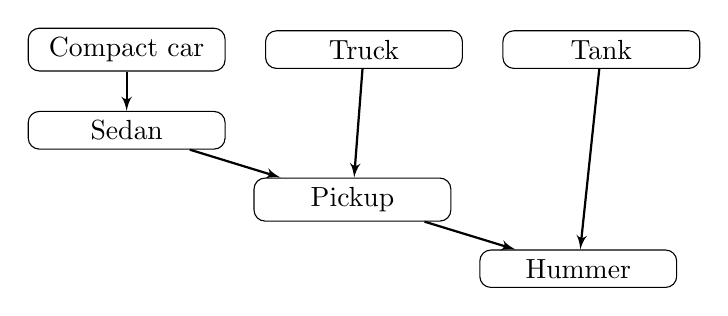
\begin{tikzpicture}
      [cars/.style={rectangle,draw=black,rounded corners,minimum width=2.5cm,node distance=0.5cm}]
      % place nodes
      \node[cars] (compact) {Compact car};
      \node[cars] (sedan) [below=of compact] {Sedan};
      \node[cars] (truck) [right=of compact] {Truck};
      \node[cars] (pickup) [below right= of sedan] {Pickup};
      \node[cars] (tank) [right=of truck] {Tank};
      \node[cars] (hummer) [below right= of pickup] {Hummer};
      % add edges
      \draw [-latex',thick] (compact) -- (sedan);
      \draw [-latex',thick] (sedan) -- (pickup);
      \draw [-latex',thick] (truck) -- (pickup);
      \draw [-latex',thick] (tank) -- (hummer);
      \draw [-latex',thick] (pickup) -- (hummer);
    \end{tikzpicture}
    \label{fig:car-hierarchy}
  }
  \hspace*{0.5cm}
  \subfloat[]{
    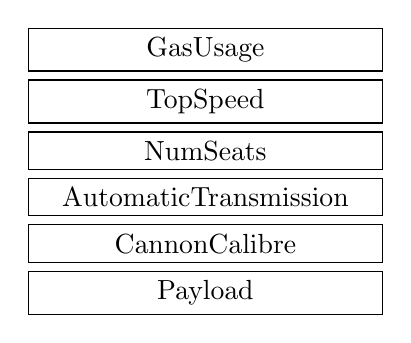
\begin{tikzpicture}
      [propertyBox/.style={rectangle,draw=black,minimum width=4.5cm,node distance=0.1cm}]
      \node[propertyBox] (gasUsage) {GasUsage};
      \node[propertyBox] (speed) [below=of gasUsage] {TopSpeed};
      \node[propertyBox] (seats) [below=of speed] {NumSeats};
      \node[propertyBox] (automatic) [below=of seats] {AutomaticTransmission};
      \node[propertyBox] (calibre) [below=of automatic] {CannonCalibre};
      \node[propertyBox] (payload) [below=of calibre] {Payload};
    \end{tikzpicture}
    \label{fig:car-propertynames}
  }
  \caption{\textbf{(a)}~A possible property inheritance graph for
    various kinds of cars.  The lower nodes inherit from higher ones;
    Inherited properties from nodes on the right take precedence over the
    properties defined on the left. \textbf{(b)}~Property names
    which make sense for at least one of the car types of (a).}
\end{figure}

Using the \Dumux property system, this inheritance hierarchy is
defined by:
\begin{lstlisting}[name=propsyscars,style=DumuxCode]
#include <dumux/common/propertysystem.hh>
#include <iostream>

namespace Dumux {
namespace Properties {
namespace TTag{
struct CompactCar {};
struct Truck {};
struct Tank {};

struct Sedan { using InheritsFrom = std::tuple<CompactCar>; };
struct Pickup { using InheritsFrom = std::tuple<Truck, Sedan>; };
struct HummerH1 { using InheritsFrom = std::tuple<Tank, Pickup>; };
}}} // end namespace TTag
\end{lstlisting}

Figure \ref{fig:car-propertynames} lists a few property names which
make sense for at least one of the nodes of Figure
\ref{fig:car-hierarchy}. These property names can be declared as
follows:
\begin{lstlisting}[name=propsyscars,style=DumuxCode]
template<class TypeTag, class MyTypeTag>
struct TopSpeed { using type = UndefinedProperty; }; // [km/h]
template<class TypeTag, class MyTypeTag>
struct NumSeats { using type = UndefinedProperty; }; // []
template<class TypeTag, class MyTypeTag>
struct CanonCaliber { using type = UndefinedProperty; }; // [mm]
template<class TypeTag, class MyTypeTag>
struct GasUsage { using type = UndefinedProperty; }; // [l/100km]
template<class TypeTag, class MyTypeTag>
struct AutomaticTransmission { using type = UndefinedProperty; }; // true/false
template<class TypeTag, class MyTypeTag>
struct Payload { using type = UndefinedProperty; }; // [t]
\end{lstlisting}

\noindent
So far, the inheritance hierarchy and the property names are completely
separate. What is missing is setting some values for the property
names on specific nodes of the inheritance hierarchy. Let us assume
the following:
\begin{itemize}
\item For a compact car, the top speed is the gas usage in $\unitfrac{l}{100km}$
  times $30$, the number of seats is $5$ and the gas usage is
  $\unitfrac[4]{l}{100km}$.
\item A truck is by law limited to $\unitfrac[100]{km}{h}$ top speed, the number
  of seats is $2$, it uses $\unitfrac[18]{l}{100km}$ and has a cargo payload of
  $\unit[35]{t}$.
\item A tank exhibits a top speed of $\unitfrac[60]{km}{h}$, uses $\unitfrac[65]{l}{100km}$
  and features a $\unit[120]{mm}$ diameter canon
\item A sedan has a gas usage of $\unitfrac[7]{l}{100km}$, as well as an automatic
  transmission, in every other aspect it is like a compact car.
\item A pick-up truck has a top speed of $\unitfrac[120]{km}{h}$ and a payload of
  $\unit[5]{t}$. In every other aspect it is like a sedan or a truck but if in
  doubt, it is more like a truck.
\item The Hummer-H1 SUV exhibits the same top speed as a pick-up
  truck.  In all other aspects it is similar to a pickup and a tank,
  but, if in doubt, more like a tank.
\end{itemize}

\noindent
Using the \Dumux property system, these assumptions are formulated
using
\begin{lstlisting}[name=propsyscars,style=DumuxCode]
template<class TypeTag>
struct TopSpeed<TypeTag, TTag::CompactCar>
{static constexpr int value = getPropValue<TypeTag, Properties::GasUsage>() * 30};

template<class TypeTag>
struct NumSeats<TypeTag, TTag::CompactCar> { static constexpr int value = 5; };

template<class TypeTag>
struct GasUsage<TypeTag, TTag::CompactCar> { static constexpr int value = 4; };

template<class TypeTag>
struct TopSpeed<TypeTag, TTag::Truck> { static constexpr int value = 100; };

template<class TypeTag>
struct NumSeats<TypeTag, TTag::Truck> { static constexpr int value = 2; };

template<class TypeTag>
struct GasUsage<TypeTag, TTag::Truck> { static constexpr int value = 18; };

template<class TypeTag>
struct Payload<TypeTag, TTag::Truck> { static constexpr int value = 35; };

template<class TypeTag>
struct TopSpeed<TypeTag, TTag::Tank> { static constexpr int value = 60; };

template<class TypeTag>
struct GasUsage<TypeTag, TTag::Tank> { static constexpr int value = 65; };

template<class TypeTag>
struct CanonCaliber<TypeTag, TTag::Tank> { static constexpr int value = 120; };

template<class TypeTag>
struct GasUsage<TypeTag, TTag::Sedan> { static constexpr int value = 7; };

template<class TypeTag>
struct AutomaticTransmission<TypeTag, TTag::Sedan> { static constexpr bool value = true; };

template<class TypeTag>
struct TopSpeed<TypeTag, TTag::Pickup> { static constexpr int value = 120; };

template<class TypeTag>
struct Payload<TypeTag, TTag::Pickup> { static constexpr int value = 5; };

template<class TypeTag>
struct TopSpeed<TypeTag, TTag::HummerH1>
{static constexpr int value = getPropValue<TypeTag, TTag::Pickup::TopSpeed<TypeTag>>();};
\end{lstlisting}

\noindent
Now property values can be retrieved and some diagnostic messages can
be generated. For example
\begin{lstlisting}[name=propsyscars,style=DumuxCode]
int main()
{
    std::cout << "top speed of sedan: " << getPropValue<Properties::TTag::Sedan, Properties::TopSpeed>() << "\n";
    std::cout << "top speed of truck: " << getPropValue<Properties::TTag::Truck, Properties::TopSpeed>() << "\n";
}
\end{lstlisting}
will yield the following output:
\begin{lstlisting}[style=Bash, basicstyle=\ttfamily\scriptsize\let\textcolor\textcolordummy]
$ top speed of sedan: 210
$ top speed of truck: 100
\end{lstlisting}

\subsection{Property Values}
To get the value of a property use:
\begin{description}
\item[\texttt{{\small getPropValue:}}]
Always returns the \emph{compile-time} specified value of the property.
\end{description}

\section{Grid Handling}
\label{sec:gridhandling}

This section summarizes some ideas about grid generation and grids that can be used by \Dumux. There are
several external grid generates available which can be used. The output files of these generators need
usually conversion into the Dune Grid Format (DGF), or some other format which can be read in by \Dune.
We intend to give brief ideas how to work with external grids. However, this list is not complete.

\subsection{DGF}
Most of our \Dumux tests and tutorials use the Dune Grid Format (DGF) to read in grids. A detailed description
of the DGF format and some examples can be found in the \Dune doxygen documentation
\textbf{(Modules $\rightarrow$ I/O $\rightarrow$ Dune Grid Format (DGF)}). To generate larger or more
complex DGF files, we recommend to write your own scripts, e.g in C++, Matlab or Python.

The DGF format can also used to read in spatial parameters defined on the grid. These parameters can
be defined on nodes as well as on the elements. An example for predefined parameters on a grid is
the \texttt{test\_boxco2} or \texttt{test\_cco2} in the  \texttt{dumux/test/co2} folder.

% Inside \Dumux, the \texttt{DGFGridCreater} is set by default and doesn't need to be set your problem file.


\subsection{GMSH}


\subsection{Petrel}
Grids from Petrel (in ASCII format with the extension *.GRDECL) can be imported into \Dumux in two ways:
  \begin{enumerate}
  \item Using the GRDECL format directly with the help of the grid-manager \texttt{dune-cornerpoint}.
  \item Converting the GRDECL file into the DGF format.
  \end{enumerate}
The fist options requires the installation of \texttt{dune-cornerpoint} along with its dependencies. Set the property \texttt{Grid} to \texttt{Dune::CpGrid} in your problem file. 

The second option has the advantage that you end up with a DGF which can then be used with any grid-manager (\texttt{dune-alugrid}, \texttt{UG} etc.) You also have to install \texttt{dune-cornerpoint}. Additionally you have to modify the converter \texttt{grdecl2vtu} found in \texttt{dune-cornerpoint/examples} to also write a DGF. To do so you have to:
\begin{itemize}
 \item Include the \texttt{dgfwriter.hh} found in \texttt{dune-grid/dune/grid/io/file/dgfparser}
 \item Create an object of the \texttt{Dune::DGFWriter} and call the its function \texttt{write()} within the \texttt{main} function for example after the \texttt{vtkwriter()} is called: 
\begin{lstlisting}[style=DumuxCode]
Dune::DGFWriterParam<CpGrid::LeafGridView> dgfWriter(grid.leafView()))
dgfWriter.write(fnamebase + ".dgf")
\end{lstlisting} 
\end{itemize}
Material parameters for elements with Petrel specific keywords like \texttt{PORO} are parsed by the converter \texttt{grdecl2vtu} (see the \texttt{main} function). They are available as vectors within the \texttt{main} function. The main GRDECL file with the coordinates must include the GRDECL files of the parameters, if for example the parameters are not already included, include the file bearing your parameter in your main GRDECL file:
\begin{lstlisting}
INCLUDE
'PARAMETER_X.GRDECL'
/
\end{lstlisting} 
To add the parameters to your DGF you have to make changes to the header \texttt{dgfwriter.hh} such that they are passed as arguments of the \texttt{write()} function and written after each element (modify \texttt{writeElement()} and internal \texttt{write()} functions accordingly). Take caution that you stick to the correct DGF syntax (see \textbf{Modules $\rightarrow$ I/O $\rightarrow$ Dune Grid Format (DGF)} for reference). 





\subsection{ArtMesh}
\href{http://www.topologica.org/toplog/wp/}{ArtMesh} is a 3D mesh generation software. It has its own mesh file format
which can be read by \Dumux via the ArtGridCreator. Traditionally it was used within \Dumux for fracture simulations with
the discrete fracture matrix model (\texttt{2pdfm}). A detailed description of the fracture network creation and gridding
can be found for example in the dissertation of \href{http://elib.uni
-stuttgart.de/opus/frontdoor.php?source_opus=8047&la=de}{Tatomir}, pp. 68.

\subsection{ICEM}
\todo[inline]{Detailierte Beschreibung im Wiki? Links entfernen, die nicht funktionieren. Text überarbeiten. (Natalie)}
For complex geometries a graphical tool to create grids might be appropriate. One possibility to mesh for example CAD
geometry data is the commercial software \href{http://www.ansys.com/Products/Other+Products/ANSYS+ICEM+CFD/}{ANSYS ICEM
CFD}. A very detailed, but outdated description can be found at the LH2 internal wiki. A more recent best practice guide is available at
\url{XXX}. At LH2 exists a script which converts the ICEM mesh into the DGF.


\bibliographystyle{plainnat}
\bibliography{dumux-handbook}
\printindex
\end{document}
